\documentclass[12pt,letterpaper]{article}

% Informe universitario con formato institucional del proyecto.
\usepackage[utf8]{inputenc}
\usepackage[T1]{fontenc}
\usepackage[spanish,es-tabla]{babel}
\usepackage{newtxtext,newtxmath}
\usepackage[letterpaper,margin=1in]{geometry}
\usepackage{setspace}
\doublespacing
\usepackage{indentfirst}
\setlength{\parindent}{0.5in}
\usepackage{graphicx}
\usepackage{booktabs,tabularx,longtable,array}
\usepackage{caption}
\captionsetup[table]{labelfont=bf,textfont=it,justification=raggedright,singlelinecheck=false,skip=4pt}
\captionsetup[figure]{labelfont=bf,textfont=it,justification=raggedright,singlelinecheck=false,skip=4pt}
\usepackage{amsmath}
\usepackage{enumitem}
\usepackage{csquotes}
\usepackage[style=authoryear,backend=biber,sorting=nyt]{biblatex}
\addbibresource{referencias.bib}
\usepackage{fancyhdr}
\usepackage{titlesec}
\usepackage{tocloft}
\usepackage[hidelinks,plainpages=false,hypertexnames=false]{hyperref}
\hypersetup{
  pdftitle={Limpieza: dataset persona.csv},
  pdfauthor={Julio Nelson Arias Cruz},
  pdfsubject={Informe de proyecto de Data Mining DAT-253},
  pdfkeywords={minería de datos, persona.csv}
}

\pagestyle{fancy}
\fancyhf{}
\fancyhead[R]{\thepage}
\setlength{\headheight}{15pt}
\renewcommand{\headrulewidth}{0pt}
\fancypagestyle{preliminar}{\fancyhf{}\fancyhead[R]{\thepage}\renewcommand{\headrulewidth}{0pt}}
\titleformat{\section}{\normalfont\bfseries\large}{\thesection.}{0.6em}{}
\titleformat{\subsection}{\normalfont\bfseries\normalsize}{\thesubsection.}{0.6em}{}
\titleformat{\subsubsection}{\normalfont\bfseries\itshape\normalsize}{\thesubsubsection.}{0.6em}{}
\renewcommand{\cftsecleader}{\cftdotfill{\cftdotsep}}
\setlength{\emergencystretch}{3em}

\begin{document}

% Carátula basada en la referencia institucional existente en informe/main.tex.
\begin{titlepage}
  \centering
  {\Large\bfseries UNIVERSIDAD MAYOR DE SAN ANDRÉS\\[0.3cm]}
  {\large\bfseries FACULTAD DE CIENCIAS PURAS Y NATURALES\\[0.2cm]}
  {\large\bfseries CARRERA DE INFORMÁTICA\\[0.2cm]}
  {\large DATA MINING (DAT-253)\\[0.4cm]}
  \vspace*{0.25in}
  
\includegraphics[width=0.31\textwidth]{Logo_Umsa.png}\\[0.2cm]
  {\Large\bfseries INFORME DE PROYECTO\\[0.25cm]}
  {\large\bfseries PREPARACIÓN DEL DATASET \texttt{persona.csv}\\[0.35cm]}

  {\footnotesize\singlespacing
    \textbf{Repositorio GitHub:} \url{https://github.com/JulioArias7200/projectFinalDM.git}\\[0.15cm]
    \textbf{Plataforma Web en Producción:} \url{https://projectfinaldm.onrender.com/dashboard/}\\[0.4cm]
  }

  {\normalsize
    \textbf{Estudiante:}\\
    Julio Nelson Arias Cruz\\[0.20cm]
    La Paz -- Bolivia\\
    2026
  }
\end{titlepage}

\pagenumbering{roman}
\setcounter{page}{2}
\thispagestyle{preliminar}
\noindent\textbf{\large Resumen}\par
\noindent
Este informe presenta la preparación, auditoría de calidad y análisis descriptivo de \texttt{data/persona.csv}, microdato sociodemográfico oficial de la Encuesta de Hogares de Bolivia considerado por el proyecto. El archivo de origen contiene 39.497 registros y 275 columnas, con una huella criptográfica SHA-256 verificada e inmutable. El resultado analítico se generó como una versión maestra inmutable (\texttt{persona\_clean\_master.parquet} y \texttt{.csv}), reteniendo íntegramente las 39.497 filas y 275 variables, acompañada de 11 vistas temáticas especializadas por población elegible, con trazabilidad exhaustiva en manifiestos y catálogo JSON local con reemplazo atómico, sin dependencia de motores externos como PostgreSQL.

La metodología aplicó reglas de calidad estrictamente respaldadas: validación y tipado de la clave primaria compuesta \texttt{(folio, nro)} (39.497 tuplas únicas, cero duplicados); taxonomía diferenciada de ausencias para respetar los 5,48 millones de tokens \texttt{NA} correspondientes a saltos legítimos del cuestionario; corrección semántica de frontera física en la regla S-01 (reasignación a \texttt{NA} de 3 celdas con jornadas semanales superiores a 168 horas físicas en \texttt{phrs}, \texttt{shrs} y \texttt{tothrs}); y normalización acotada a minúsculas en la regla S-02 (12.516 celdas en 13 variables de respuesta abierta tipo ``Especifique''). Se descartó la eliminación destructiva de variables por umbral del 80\% (regla L-80), tratándose como alerta informativa.

La suite del sistema analítico incluye una aplicación web en Flask que consume la versión validada por catálogo JSON, presentando resúmenes de calidad, perfiles de los 11 universos temáticos y un mapa interactivo de Bolivia con división oficial de los 9 departamentos. Se documenta la distribución exacta observada de la muestra ($N = 39.497$ personas y $N_{\text{hog}} = 12.718$ hogares), delimitando indicadores de salud, educación, empleo e ingresos para uso descriptivo riguroso.

\vspace{0.3cm}
\noindent\textbf{Palabras clave:} minería de datos, calidad de datos, limpieza trazable, encuesta de hogares, análisis descriptivo.

\newpage
\thispagestyle{preliminar}
\tableofcontents
\newpage
\thispagestyle{preliminar}
\listoftables
\newpage
\thispagestyle{preliminar}
\listoffigures

\newpage
\pagenumbering{arabic}
\setcounter{page}{1}

\section{Introducción}

Los proyectos de minería de datos requieren más que ejecutar algoritmos de aprendizaje automático: necesitan comprender a profundidad la naturaleza de las fuentes, auditar rigurosamente su calidad, preparar los microdatos mediante reglas explícitas y reproducibles, y comunicar con honestidad las limitaciones epistemológicas de cada resultado. La metodología estándar CRISP-DM (\textit{Cross-Industry Standard Process for Data Mining}) y el marco KDD (\textit{Knowledge Discovery in Databases}) conciben un ciclo iterativo estructurado que vincula estrechamente la comprensión del negocio o dominio, la exploración y preparación de los datos, el modelado, la evaluación y el despliegue operativo \parencite{chapman2000crisp, fayyad1996data}. En el análisis de microdatos sociodemográficos procedentes de encuestas por muestreo probabilístico, esta rigurosidad es indispensable: códigos categóricos, valores especiales de no respuesta y filtros o saltos condicionales del cuestionario pueden inducir a conclusiones gravemente distorsionadas si se procesan como atributos numéricos convencionales o si se aplican recetas simplistas de imputación masiva.

El presente proyecto aborda el procesamiento integral de \texttt{data/persona.csv}, archivo de microdatos de personas de la Encuesta de Hogares de Bolivia (EH2025). La estructura local observada consta de 39.497 registros individuales y 275 variables. Se cuenta con un diccionario de metadatos de referencia basado en el archivo F27 del catálogo oficial ANDA del Instituto Nacional de Estadística (INE); no obstante, el catálogo oficial declara 39.485 casos y 276 variables \parencite{ineeh2025persona}. Esta discrepancia (12 registros adicionales y variaciones en la denominación de campos) prohíbe asumir apriorísticamente que la copia de trabajo sea idéntica a la publicación oficial, exigiendo un principio de conservación y auditoría transparente sobre la fuente efectivamente analizada.

\subsection{Problema y pregunta de trabajo}
En el ámbito de la ciencia de datos aplicada a políticas públicas, el problema de limpieza no consiste simplemente en sustituir celdas vacías o eliminar observaciones atípicas. Consiste en generar una base analítica reproducible sin destruir información cuya interpretación responde al diseño muestral de la encuesta. En este contexto:
\begin{itemize}[leftmargin=0.5in]
  \item Una celda con token de ausencia (\texttt{NA}) no equivale necesariamente a un error del encuestador o una omisión del informante: con frecuencia representa una persona que legítimamente no forma parte del universo de la pregunta (por ejemplo, preguntas de empleo para menores de 7 años o de maternidad para varones).
  \item Un valor extremo en distribuciones asimétricas de ingreso o edad puede ser perfectamente plausible y no constituye un error que deba suprimirse mediante métodos de truncamiento ciego como el rango intercuartílico (IQR).
  \item Un código numérico discreto (como el departamento o la condición de actividad) no posee propiedades métricas y no admite cálculos de media o desviación estándar sin provocar un error categorial.
\end{itemize}

Frente a este escenario, la pregunta central que guía el proyecto es: \textit{¿Cómo estructurar un pipeline determinista y auditable que limpie y valide técnicamente el dataset \texttt{persona.csv}, preservando la inmutabilidad de la fuente cruda, respetando la estructura de universos muestrales y desplegando un sistema analítico interactivo en Flask con persistencia atómica en JSON local?}

\subsection{Objetivos}
El objetivo general es diseñar, ejecutar y documentar un sistema verificable de preparación, auditoría de calidad y visualización analítica de \texttt{persona.csv}, garantizando la inmutabilidad del archivo original, aplicando transformaciones semánticas trazables y estructurando 11 vistas temáticas especializadas.

Los objetivos específicos son:
\begin{enumerate}[leftmargin=0.5in]
  \item Caracterizar la estructura técnica, la integridad criptográfica (SHA-256) y la taxonomía de ausencias del archivo \texttt{data/persona.csv}.
  \item Validar la unicidad de la clave primaria compuesta \texttt{(folio, nro)} y formalizar el contrato de datos para las 275 columnas.
  \item Implementar y registrar en bitácora transaccional únicamente reglas de limpieza con fundamento físico o lingüístico verificable (reglas S-01 y S-02), preservando el esquema maestro en formato Parquet y CSV.
  \item Construir 11 vistas analíticas temáticas orientadas a subpoblaciones elegibles según los saltos del cuestionario oficial del INE.
  \item Desarrollar una aplicación web interactiva en Flask con arquitectura desacoplada, persistencia atómica en JSON local (sin base de datos relacional pesada) y un módulo geográfico interactivo de los 9 departamentos de Bolivia con datos observados exactos.
\end{enumerate}

\subsection{Alcance y delimitación}
El análisis se concentra exclusivamente en el microdato individual de \texttt{persona.csv}; no realiza fusiones con las bases complementarias de vivienda, gastos o equipamiento del hogar. Las 11 vistas temáticas generadas son proyecciones analíticas de la versión maestra y no descartan variables del esquema global. El alcance abarca preparación, auditoría, perfiles de calidad y visualización descriptiva. No se entrenan modelos de aprendizaje automático predictivo ni se efectúan inferencias poblacionales no ponderadas, en estricto cumplimiento de los supuestos del diseño muestral complejo.

\section{Fundamento teórico y metodológico}

\subsection{Minería de datos y marcos de ciclo de vida: CRISP-DM y KDD}
La minería de datos se define formalmente como la etapa no trivial dentro del proceso de Descubrimiento de Conocimiento en Bases de Datos (KDD) orientada a la identificación de patrones válidos, novedosos, potencialmente útiles y comprensibles \parencite{fayyad1996data, fayyad1996kdd}. El marco KDD divide la cadena de valor en cinco etapas secuenciales e iterativas: selección, preprocesamiento/limpieza, transformación, minería propiamente dicha y evaluación/interpretación.

Por su parte, la metodología CRISP-DM organiza el esfuerzo analítico en seis fases interconectadas: Comprensión del Negocio, Comprensión de los Datos, Preparación de los Datos, Modelado, Evaluación y Despliegue \parencite{chapman2000crisp}. En proyectos fundamentados en microdatos oficiales, la literatura metodológica del curso de Minería de Datos subraya que más del 70\% del esfuerzo técnico reside en la fase de \textit{Preparación de Datos} \parencite{umsa2026curso}. Un modelado predictivo prematuro sobre variables con errores de tipado o saltos de encuesta malinterpretados produce artefactos espurios y perpetúa sesgos estructurales. Por consiguiente, este proyecto delimita su alcance a consolidar un ciclo de preparación, auditoría de calidad y entrega analítica inmutable, garantizando bases firmes para futuros algoritmos de agrupamiento, clasificación o inferencia.

\subsection{Principios teóricos de preparación de datos y calidad}
El sustento técnico de este trabajo se articula a partir de los principios desarrollados en los módulos temáticos de la materia \parencite{umsa2026curso}:

\begin{enumerate}[leftmargin=0.5in]
  \item \textbf{Tipología y escalas de medición (Capítulo 2):} Separación estricta entre identificadores relacionales (\texttt{folio}, \texttt{nro}), variables nominales codificadas (\texttt{s01a\_01}, \texttt{depto}), ordinales (\texttt{niv\_ed}) y magnitudes cuantitativas (\texttt{edad}, \texttt{phrs}, \texttt{ylab}). Se prohíbe explícitamente calcular medias sobre variables categóricas o interpretar códigos numéricos sin diccionario.
  \item \textbf{Estadística descriptiva y detección de anomalías (Capítulo 3):} Empleo del rango intercuartílico (IQR), cuantiles y medidas de dispersión no como herramientas de eliminación destructiva de registros, sino como alertas diagnósticas para orientar la auditoría humana especializada.
  \item \textbf{Tratamiento de valores faltantes y universos condicionales (Capítulo 5):} Clasificación formal de las ausencias. Se distingue entre no respuesta aleatoria (omisión de respuesta) y no respuesta estructural (resultado de un salto legítimo del cuestionario). Se prohíbe la imputación de medias o modas globales sobre campos condicionales.
  \item \textbf{Aseguramiento de la calidad y ciclo de vida de datos (Capítulo 11):} Implementación de controles censales, registro de cambios en bitácoras \textit{append-only} y preservación de la reproducibilidad científica mediante verificación criptográfica de artefactos intermedios y finales.
  \item \textbf{Límites de la inferencia estadística (Capítulo 4):} Distinción rigurosa entre estadísticos observados en la muestra ($n = 39.497$) y estimaciones paramétricas poblacionales ($N \approx 12,4\text{ millones}$). Cualquier cálculo inferencial generalizable requiere incorporar el diseño muestral complejo (estratificación y ponderadores \texttt{factor}).
\end{enumerate}

\subsection{Trazabilidad, persistencia atómica y gobernanza en JSON}
En concordancia con las restricciones de diseño arquitectónico del proyecto, se descartó el uso de sistemas de gestión de bases de datos relacionales pesadas como PostgreSQL. En su lugar, se adoptó una arquitectura ligera, portable y desacoplada basada en archivos inmutables en disco (Parquet/CSV) y persistencia de catálogos mediante documentos JSON locales con sustitución atómica. 

Bajo este esquema, una versión candidata no se hace visible para la interfaz web hasta que supera todas las compuertas de validación de integridad (esquema, recuento censal y verificación de hashes). Toda modificación de celdas queda registrada con actor, regla, valor anterior y nuevo en una bitácora append-only, asignando al despliegue el estado técnico explícito \texttt{published\_internal\_with\_semantic\_limitations}, lo que garantiza honestidad intelectual al delimitar qué variables cuentan con respaldo semántico confirmado y cuáles permanecen en estado de revisión.

\section{Metodología}

\subsection{Diseño del estudio y fuente de datos}
Se desarrolló un estudio tecnológico y analítico de carácter descriptivo, cuantitativo y auditable sobre el microdato oficial \texttt{data/persona.csv}. El archivo original contiene 39.497 filas y 275 atributos, ocupando 34.568.646 bytes con una huella criptográfica SHA-256 verificada:
\begin{quote}\small\ttfamily
568e82e3039d991a1ee0d8e2056448f8c465c03ffa838330c4f1522dd77bddc8
\end{quote}
Como referencia semántica auxiliar se utilizó el diccionario de datos oficial del INE para el formulario F27 (EH2025\_Persona), estableciendo puentes entre variables sin alterar la fuente original.

\subsection{Etapas del procedimiento operativo}
Siguiendo las fases del ciclo CRISP-DM y KDD, el procedimiento se estructuró en siete etapas reproducibles (ilustradas en la figura \ref{fig:crisp_kdd}):

\begin{enumerate}[leftmargin=0.5in]
  \item \textbf{Comprensión y contrato de datos:} Formalización del esquema de 275 variables, definición de tipos admisibles, clasificación de campos sensibles y estipulación de inmutabilidad sobre el raw.
  \item \textbf{Ingesta e inspección estructural:} Lectura controlada en modo texto para prevenir conversiones automáticas erróneas de ceros o tokens especiales; validación de encabezados únicos y anchura uniforme de registros.
  \item \textbf{Diagnóstico y perfilado multivariado:} Medición de tokens de ausencia (\texttt{""} vs. \texttt{NA} vs. \texttt{0}), cardinalidad de categorías, rangos cuantitativos e identificación de valores extremos mediante IQR.
  \item \textbf{Diseño y aprobación de reglas:} Formulación de reglas respaldadas por teoría física, lingüística o matemática, con condición, acción, universo de impacto y política de rechazo.
  \item \textbf{Preparación y ejecución controlada:} Aplicación secuencial de las reglas autorizadas, generando la versión maestra limpia (\texttt{persona\_clean\_master.parquet}) y registrando toda alteración en bitácora append-only.
  \item \textbf{Modelado por universos y derivación de vistas:} Segmentación de la población en 11 vistas temáticas especializadas basadas estrictamente en los saltos y preguntas filtro de la encuesta.
  \item \textbf{Auditoría, publicación atómica y despliegue:} Verificación censal de dimensiones y claves, persistencia de manifiestos y hashes en JSON local, y sincronización transaccional con la aplicación web Flask.
\end{enumerate}

\begin{figure}[htbp]
\centering
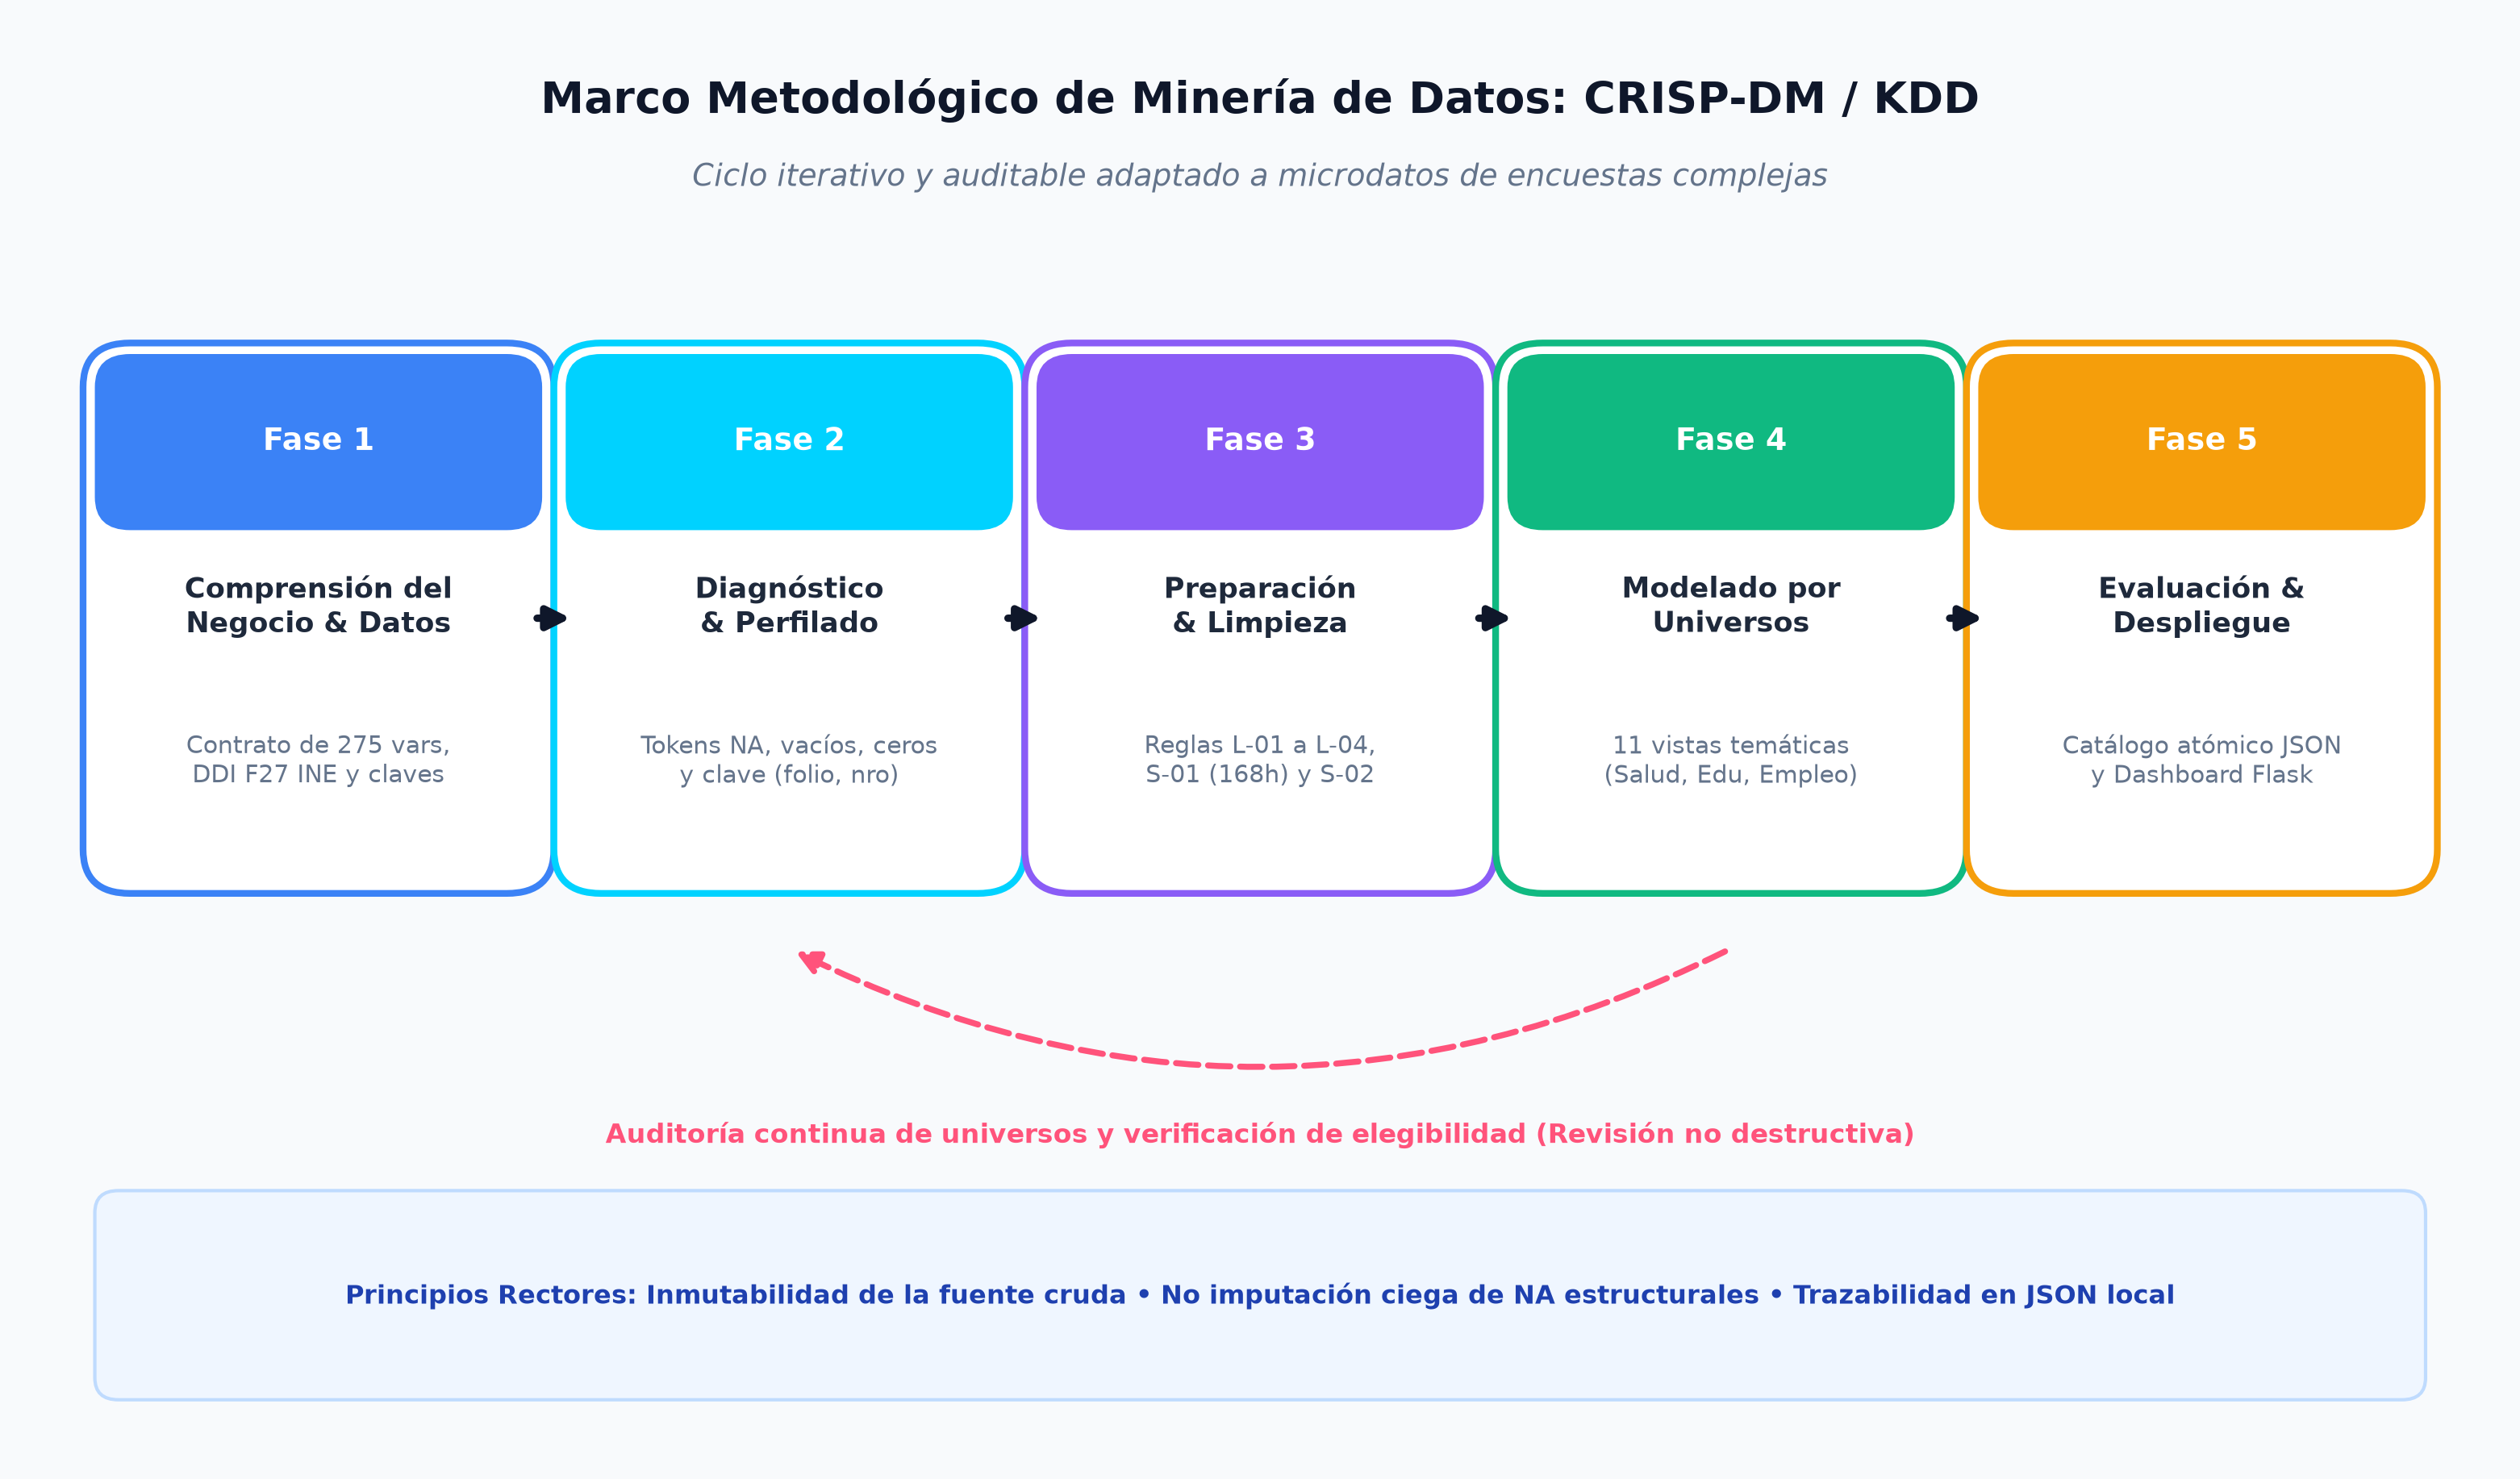
\includegraphics[width=0.98\textwidth]{figuras/fig1_metodologia_crisp_kdd.png}
\caption{Ciclo de vida metodológico CRISP-DM / KDD adaptado al proyecto}
\label{fig:crisp_kdd}
\par\vspace{3pt}\parbox{0.98\textwidth}{\footnotesize\textit{Nota.} Esquema de las cinco fases operativas del proyecto y su bucle iterativo de auditoría de universos. Elaboración propia a partir del marco teórico de Minería de Datos.}
\end{figure}

\begin{figure}[htbp]
\centering
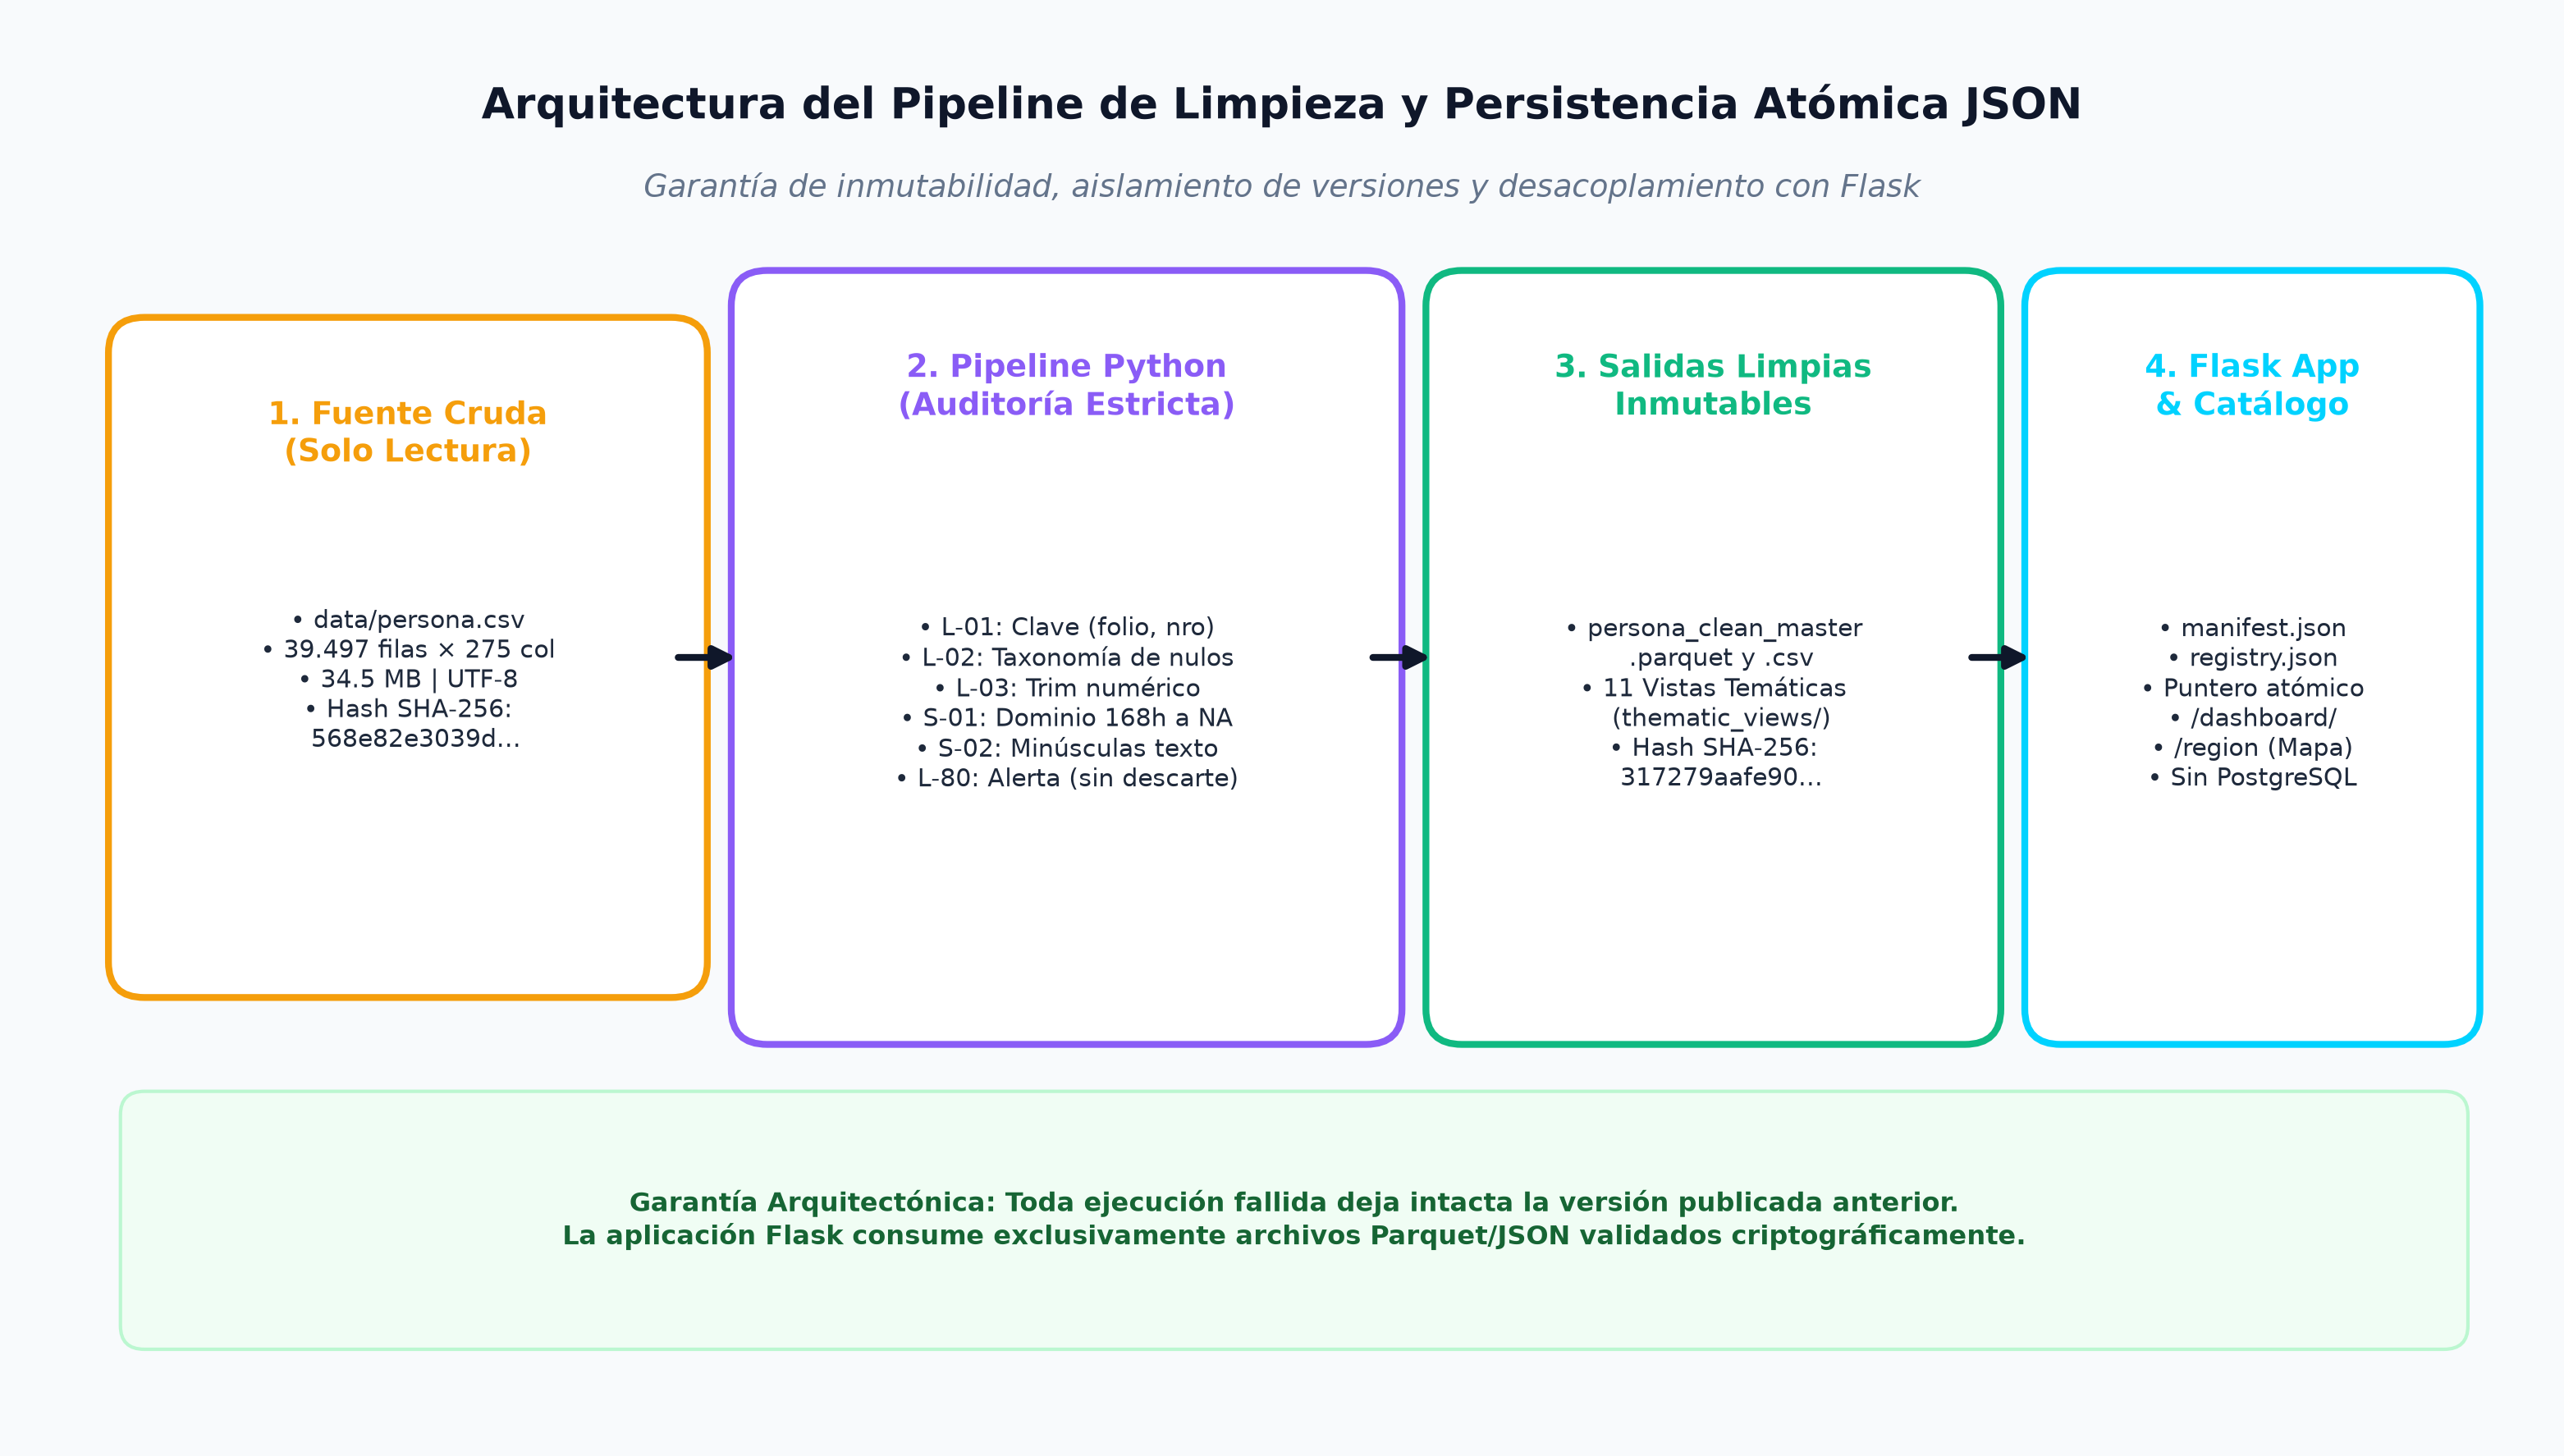
\includegraphics[width=0.98\textwidth]{figuras/fig2_arquitectura_pipeline_json.png}
\caption{Arquitectura del pipeline de limpieza, persistencia atómica JSON y desacoplamiento con Flask}
\label{fig:arquitectura_pipeline}
\par\vspace{3pt}\parbox{0.98\textwidth}{\footnotesize\textit{Nota.} Flujo de transformación que preserva la inmutabilidad de la fuente cruda, materializa el maestro Parquet y actualiza los punteros JSON locales sin gestor relacional externo.}
\end{figure}

\subsection{Catálogo de reglas de limpieza y calidad ejecutadas}
El pipeline ejecuta de manera determinista las siguientes reglas de calidad:

\begin{itemize}[leftmargin=0.5in]
  \item \textbf{Regla L-01 (Clave Primaria Compuesta):} Tipado a enteros positivos y validación estricta de unicidad sobre la tupla relacional \texttt{(folio, nro)}, confirmando que \texttt{folio} identifica la vivienda/hogar y \texttt{nro} al integrante familiar. Se comprobaron 39.497 tuplas únicas (0 duplicados y 0 vacíos).
  \item \textbf{Regla L-02 (Taxonomía de Tokens de Ausencia):} Tratamiento diferenciado de celdas vacías (\texttt{""}), tokens explícitos (\texttt{NA}) y ceros legítimos (\texttt{0}), evitando la colisión o imputación prematura de valores fuera de universo.
  \item \textbf{Regla L-03 (Normalización de Espacios - Trim):} Eliminación de espacios en blanco residuales en las 256 columnas numéricas y códigos categóricos, preservando sin alteración el texto libre.
  \item \textbf{Regla L-04 (Validación de Dominios Categóricos):} Verificación de que variables clave cumplan los códigos oficiales del INE (\texttt{s01a\_01} $\in \{1,2\}$ para sexo, \texttt{depto} $\in \{1..9\}$ y \texttt{area} $\in \{1,2\}$). Cero anomalías detectadas.
  \item \textbf{Regla S-01 (Frontera Física en Horas Semanales):} Validación del límite biológico infranqueable de 168 horas semanales ($7 \times 24$) en variables de jornada laboral (\texttt{phrs}, \texttt{shrs}, \texttt{tothrs}). Tres registros con valores imposibles (171.5h, 180h y 192h) fueron reasignados a \texttt{NA} con registro detallado en bitácora append-only, sin suprimir las filas.
  \item \textbf{Regla S-02 (Normalización Textual Controlada):} Conversión exclusiva a minúsculas en 13 variables de respuesta abierta identificadas como campos de especificación en el diccionario, sin modificar identificadores ni categorías.
  \item \textbf{Regla L-80 (Umbral Técnico Informativo):} Mantiene como advertencia de revisión aquellas variables con más del 80\% de ausencia global, prohibiendo su exclusión destructiva del maestro para no eliminar preguntas condicionales legítimas.
\end{itemize}

\subsection{Estrategia de verificación y control muestral (QA)}
Para validar la no regresión y la integridad de las transformaciones, se implementó una suite automatizada de 16 pruebas sintéticas unitarias que verifican la retención de columnas con 100\% de ausencia, la idempotencia de los algoritmos de trim, el bloqueo preventivo ante claves duplicadas y la lectura protegida por hash SHA-256. Asimismo, se seleccionó una muestra determinista de control de 381 hogares (1.216 personas) estratificada por departamento y área para auditoría intrahogar.

\section{Resultados}

\subsection{Estructura técnica y verificación de integridad criptográfica}
La lectura inicial del archivo \texttt{data/persona.csv} mediante análisis de flujo determinó la perfecta coherencia estructural de la matriz de datos: no se encontraron encabezados duplicados, líneas incompletas ni anomalías de delimitación. En la tabla \ref{tab:estructura} se resumen las métricas básicas de integridad observadas en la copia original.

\begin{table}[htbp]
\centering
\caption{Características estructurales y verificación del archivo de entrada}
\label{tab:estructura}
\begin{tabularx}{0.88\textwidth}{Xr}
\toprule
\textbf{Parámetro de control} & \textbf{Resultado observado} \\
\midrule
Registros totales de personas ($N$) & 39.497 \\
Hogares únicos identificados ($N_{\text{hog}}$ vía \texttt{folio}) & 12.718 \\
Atributos / Columnas & 275 \\
Volumen en disco & 34.568.646 bytes \\
Codificación de caracteres & UTF-8 sin BOM \\
Encabezados duplicados o corruptos & 0 \\
Registros con anchura de campos incorrecta & 0 \\
Filas idénticas repetidas en la matriz & 0 \\
Claves primarias candidatas \texttt{(folio, nro)} duplicadas & 0 \\
\bottomrule
\end{tabularx}
\par\vspace{3pt}\parbox{0.88\textwidth}{\footnotesize\textit{Nota.} SHA-256: {\scriptsize\texttt{568e82e3039d991a1ee0d8e2056448f8c465c03ffa838330c4f1522dd77bddc8}}. Fuente: Manifiesto de ejecución local.}
\end{table}

\subsection{Diagnóstico de ausencias y refutación del descarte ciego (L-80)}
El diagnóstico cuantitativo sobre las 10.861.675 celdas del dataset reveló la presencia de 771.655 celdas exactamente vacías (\texttt{""}), 5.489.754 tokens explícitos de no respuesta (\texttt{NA}) y 1.192.066 celdas con el valor numérico legítimo \texttt{0}. 

Tal como se ilustra en la figura \ref{fig:diagnostico_ausencia} (Panel A), los tokens \texttt{NA} representan el 50,5\% de las celdas totales. Sin embargo, este volumen no traduce una mala calidad de recolección, sino la existencia de módulos del cuestionario con saltos condicionales. En una corrida preliminar histórica, la aplicación de una regla ciega de umbral al 80\% (L-80 calculada sobre todas las filas) excluyó indebidamente 125 variables. Como se demuestra en el Panel B de la figura \ref{fig:diagnostico_ausencia}, la variable de salario líquido (\texttt{s04c\_17a}) presenta 81,35\% de ausencia en la población global, pero al delimitar su universo real a las personas asalariadas elegibles ($N = 7.370$), solo 4 casos corresponden a faltantes reales (0,05\% de omisión). Por ello, el maestro definitivo retiene la totalidad de las 275 variables.

\begin{figure}[htbp]
\centering
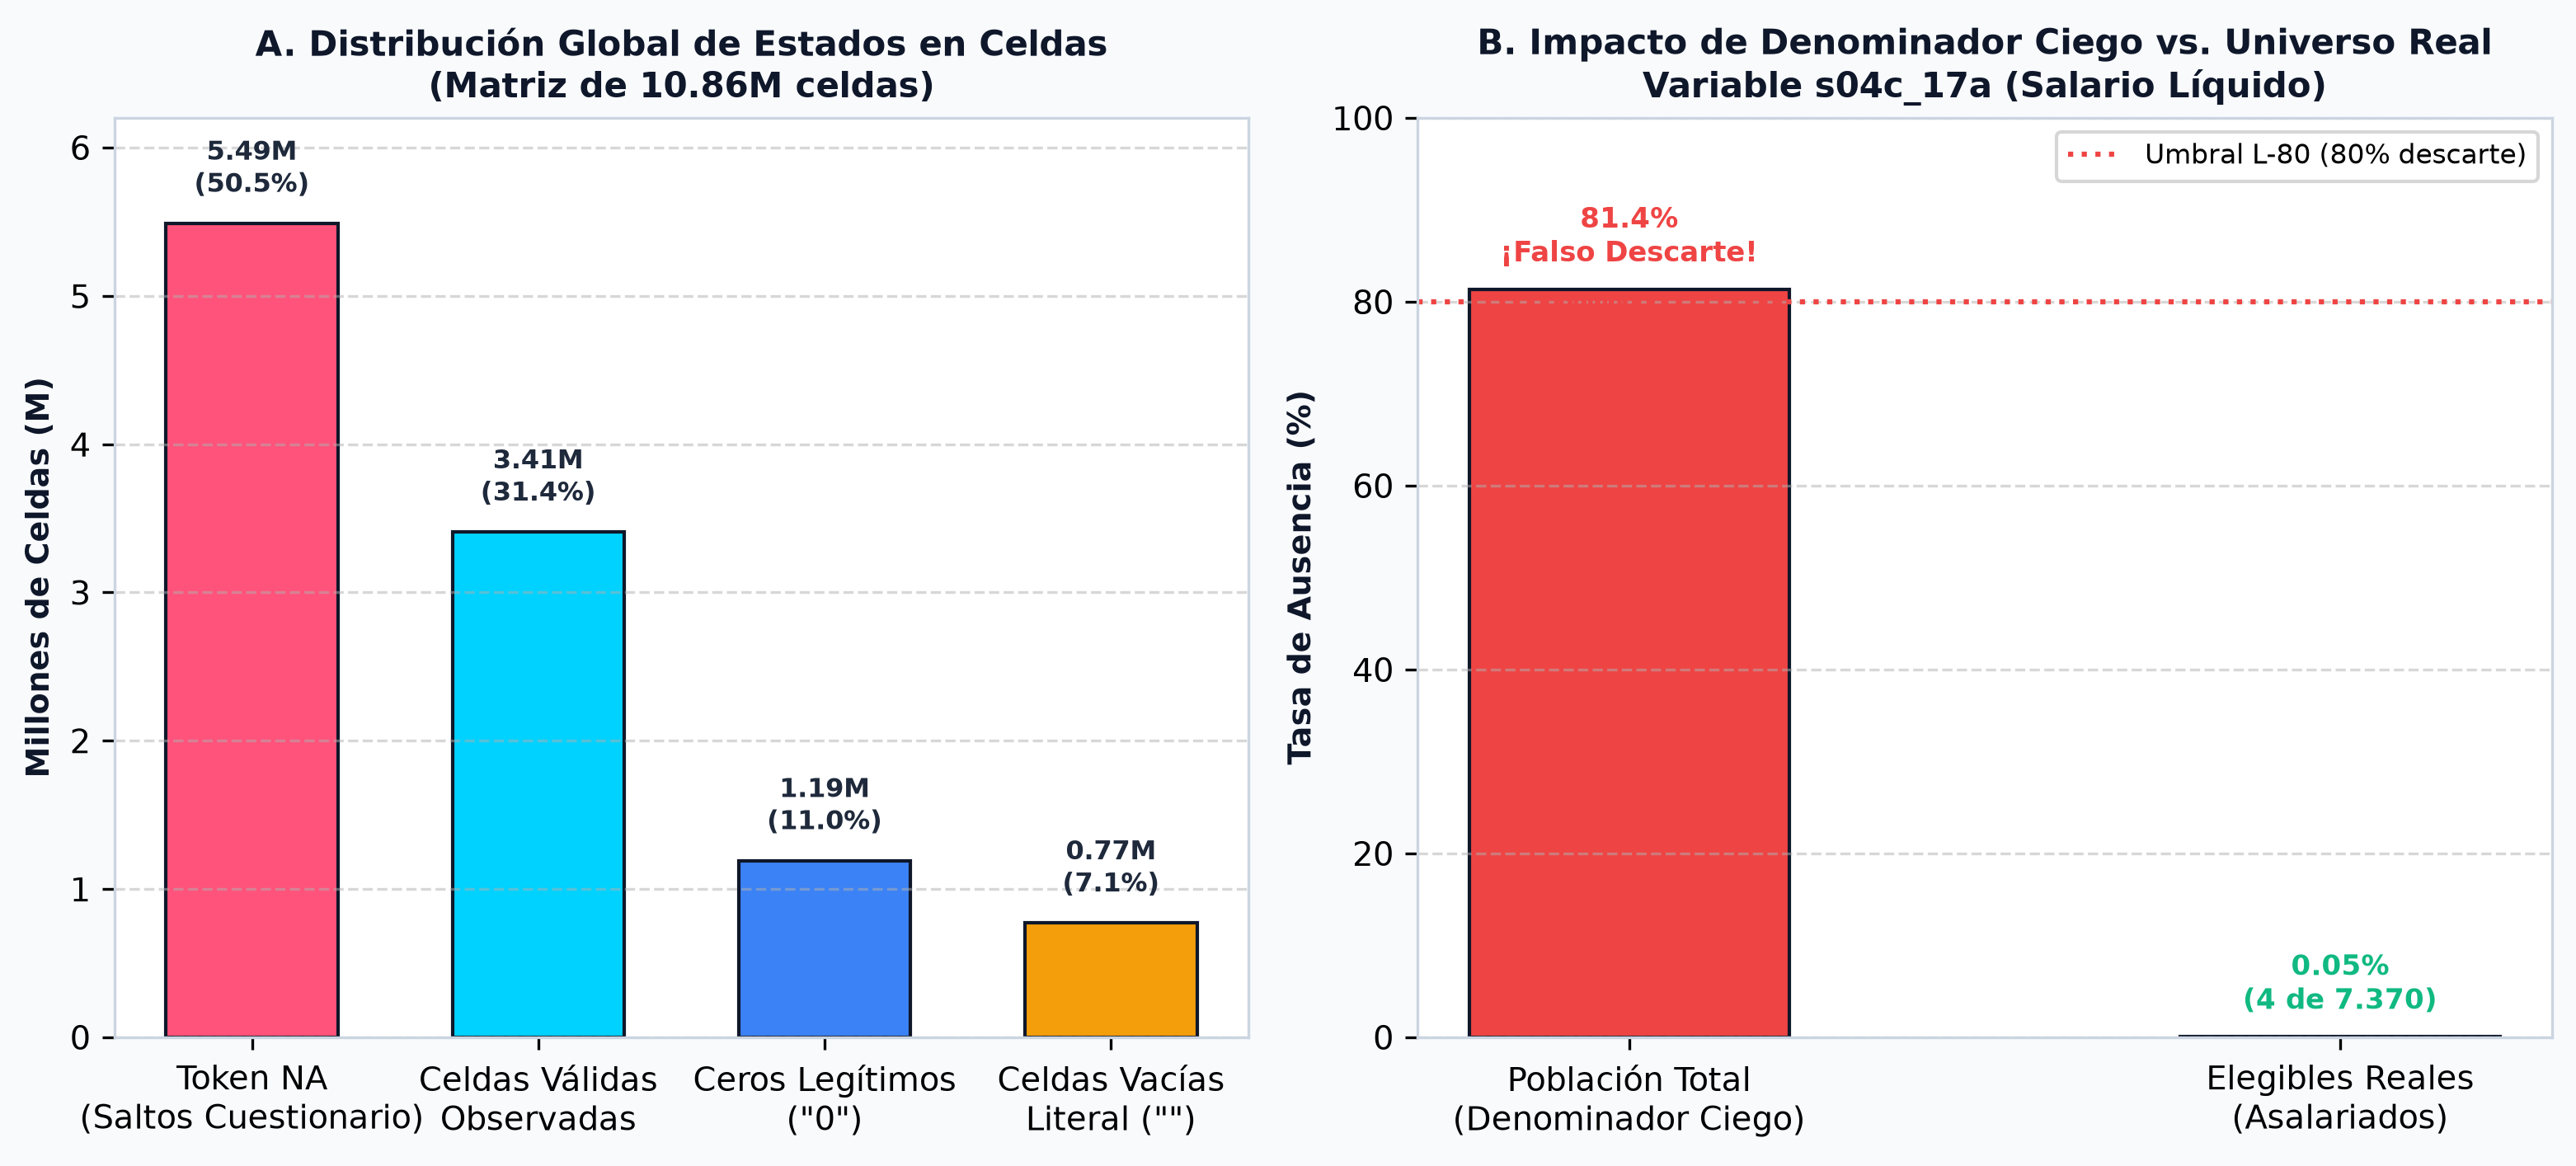
\includegraphics[width=0.98\textwidth]{figuras/fig3_diagnostico_tokens_ausencia.png}
\caption{Diagnóstico de estados de ausencia en celdas y falacia del descarte global por L-80}
\label{fig:diagnostico_ausencia}
\par\vspace{3pt}\parbox{0.98\textwidth}{\footnotesize\textit{Nota.} El panel A clasifica los 10,86 millones de celdas. El panel B demuestra cómo el 81,4\% de ausencia en salario líquido (\texttt{s04c\_17a}) se reduce a 0,05\% al evaluarse en su población elegible documentada.}
\end{figure}

\subsection{Catálogo de reglas de calidad y transformaciones trazadas}
La versión definitiva de trabajo, identificada como \texttt{\small persona-\allowbreak 317279aa\allowbreak fe9023a2}, mantiene la totalidad de los 39.497 registros y las 275 columnas tanto en formato CSV como en Apache Parquet. En la tabla \ref{tab:reglas} se sintetiza el impacto medible de cada regla de limpieza aplicada.

\begin{table}[htbp]
\centering
\caption{Catálogo consolidado de reglas de preparación y limpieza ejecutadas}
\label{tab:reglas}
\begin{tabularx}{\textwidth}{>{\raggedright\arraybackslash\small}p{1.2cm}>{\raggedright\arraybackslash\small}p{3.8cm}>{\raggedright\arraybackslash\small}p{1.7cm}>{\raggedright\arraybackslash\small}X}
\toprule
\textbf{Regla} & \textbf{Condición y fundamento} & \textbf{Impacto real} & \textbf{Efecto analítico y evidencia} \\
\midrule
\textbf{L-01} & \texttt{(folio, nro)} como clave compuesta tipada a enteros $\mathbb{Z}^+$. & 39.497 tuplas verificadas & Cero colisiones; confirma estructura de hogar y persona. \\
\textbf{L-02} & Taxonomía diferenciada entre vacío, token \texttt{NA} y cero legítimo. & 7,45M celdas clasificadas & Preservación de saltos; prohibición de imputación ciega con medias. \\
\textbf{L-03} & Trim de espacios blancos en 256 columnas numéricas y códigos. & 256 columnas normalizadas & Estandarización de tipos en Parquet sin afectar texto libre. \\
\textbf{L-04} & Verificación de códigos contra catálogo oficial DDI F27 del INE. & 100\% de conformidad & Validación de \texttt{depto} (1..9), \texttt{area} (1,2) y \texttt{s01a\_01} (1,2). \\
\textbf{S-01} & Frontera física biológica: horas semanales $\le 168$ ($7 \times 24$). & 3 celdas tratadas a \texttt{NA} & Corrección en \texttt{phrs}, \texttt{shrs}, \texttt{tothrs} (171.5h, 180h y 192h). Filas conservadas. \\
\textbf{S-02} & Normalización a minúsculas solo en texto abierto de especificación. & 12.516 celdas corregidas & Aplicada en 13 columnas específicas; claves y códigos intactos. \\
\textbf{L-80} & Monitoreo de alta ausencia técnica global ($>80\%$). & Alerta informativa & Prohíbe descarte destructivo; variables conservadas en el maestro. \\
\bottomrule
\end{tabularx}
\par\vspace{3pt}\parbox{\textwidth}{\footnotesize\textit{Nota.} El archivo maestro resultante conserva el 100\% de filas y atributos originales. Las alteraciones semánticas de la regla S-01 están registradas en \texttt{semantic\_cell\_changes\_restricted.csv}.}
\end{table}

La regla S-01 se detalla en la figura \ref{fig:auditoria_s01}: se contrastó la distribución de jornadas laborales con el límite biológico semanal, registrándose en bitácora auditable la reasignación de las 3 celdas físicamente anómalas.

\begin{figure}[htbp]
\centering
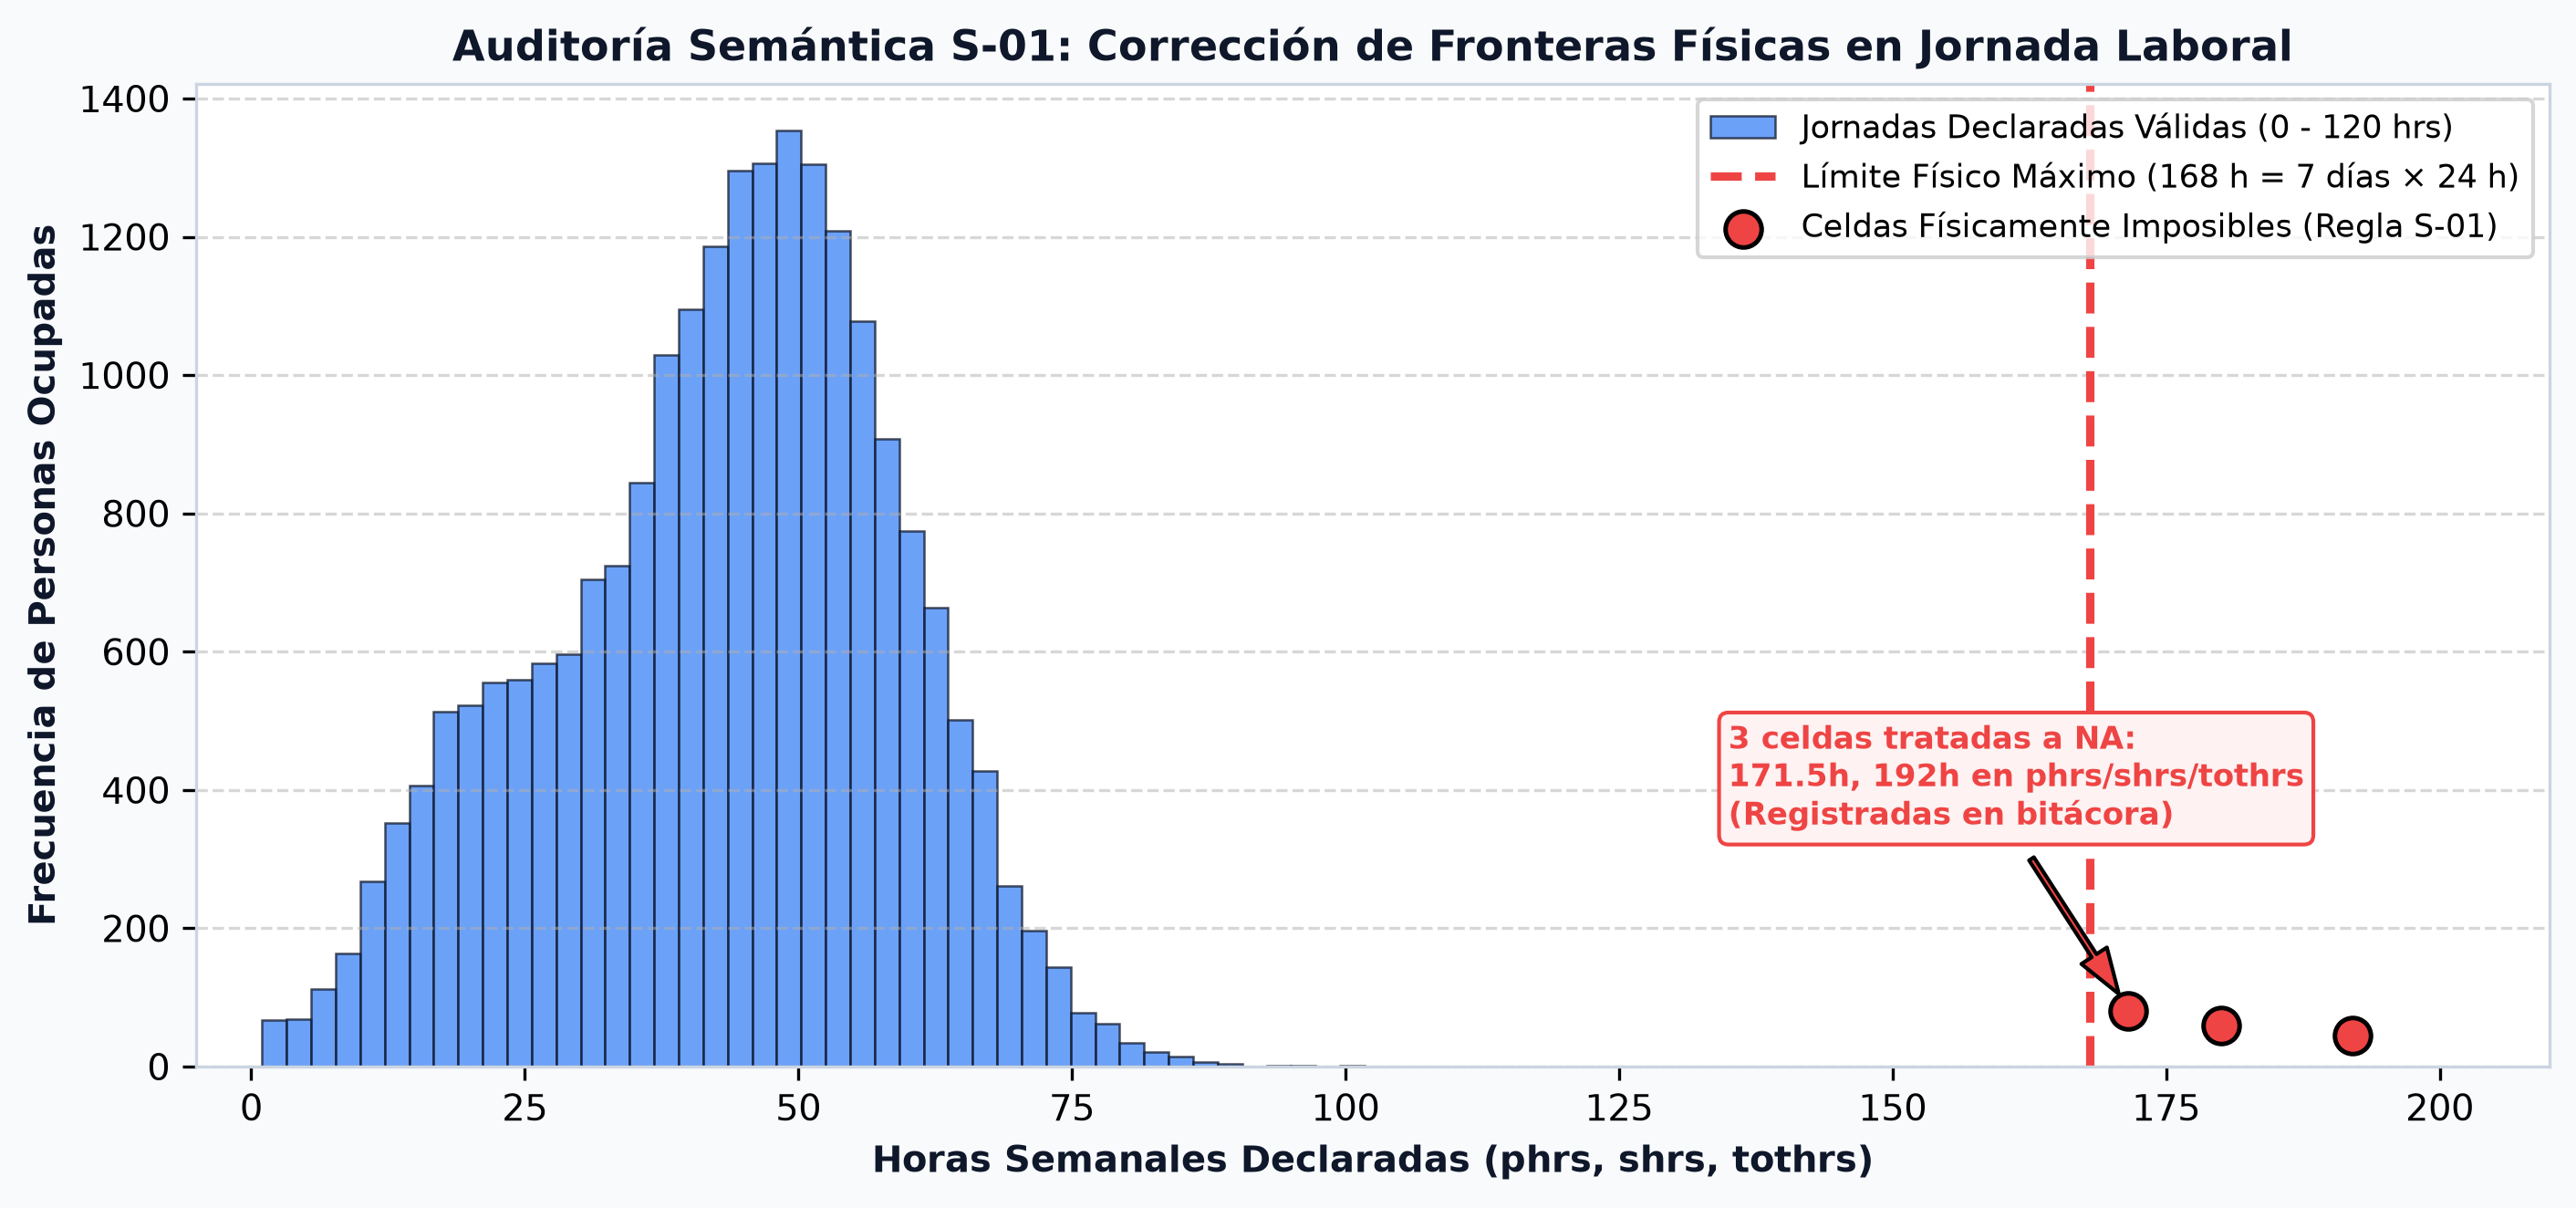
\includegraphics[width=0.92\textwidth]{figuras/fig5_auditoria_horas_semanales_s01.png}
\caption{Auditoría semántica de la regla S-01: Control de límites físicos en jornada semanal}
\label{fig:auditoria_s01}
\par\vspace{3pt}\parbox{0.92\textwidth}{\footnotesize\textit{Nota.} Distribución de horas semanales declaradas y reasignación trazable de los valores extremos imposibles ($> 168$ h) sin eliminación de observaciones.}
\end{figure}

\subsection{Delimitación territorial de la muestra por departamento}
La distribución espacial observada de los 39.497 encuestados refleja la cobertura del operativo censal en los nueve departamentos de Bolivia. En la figura \ref{fig:distribucion_departamental} se presenta el desglose según área urbana y rural. Se advierte una alta concentración urbana en los departamentos del eje central (La Paz con 86,1\%, Santa Cruz con 88,5\% y Cochabamba con 82,0\%), frente a una predominancia rural acentuada en Potosí (40,5\%) y Chuquisaca (31,5\%).

\begin{figure}[htbp]
\centering
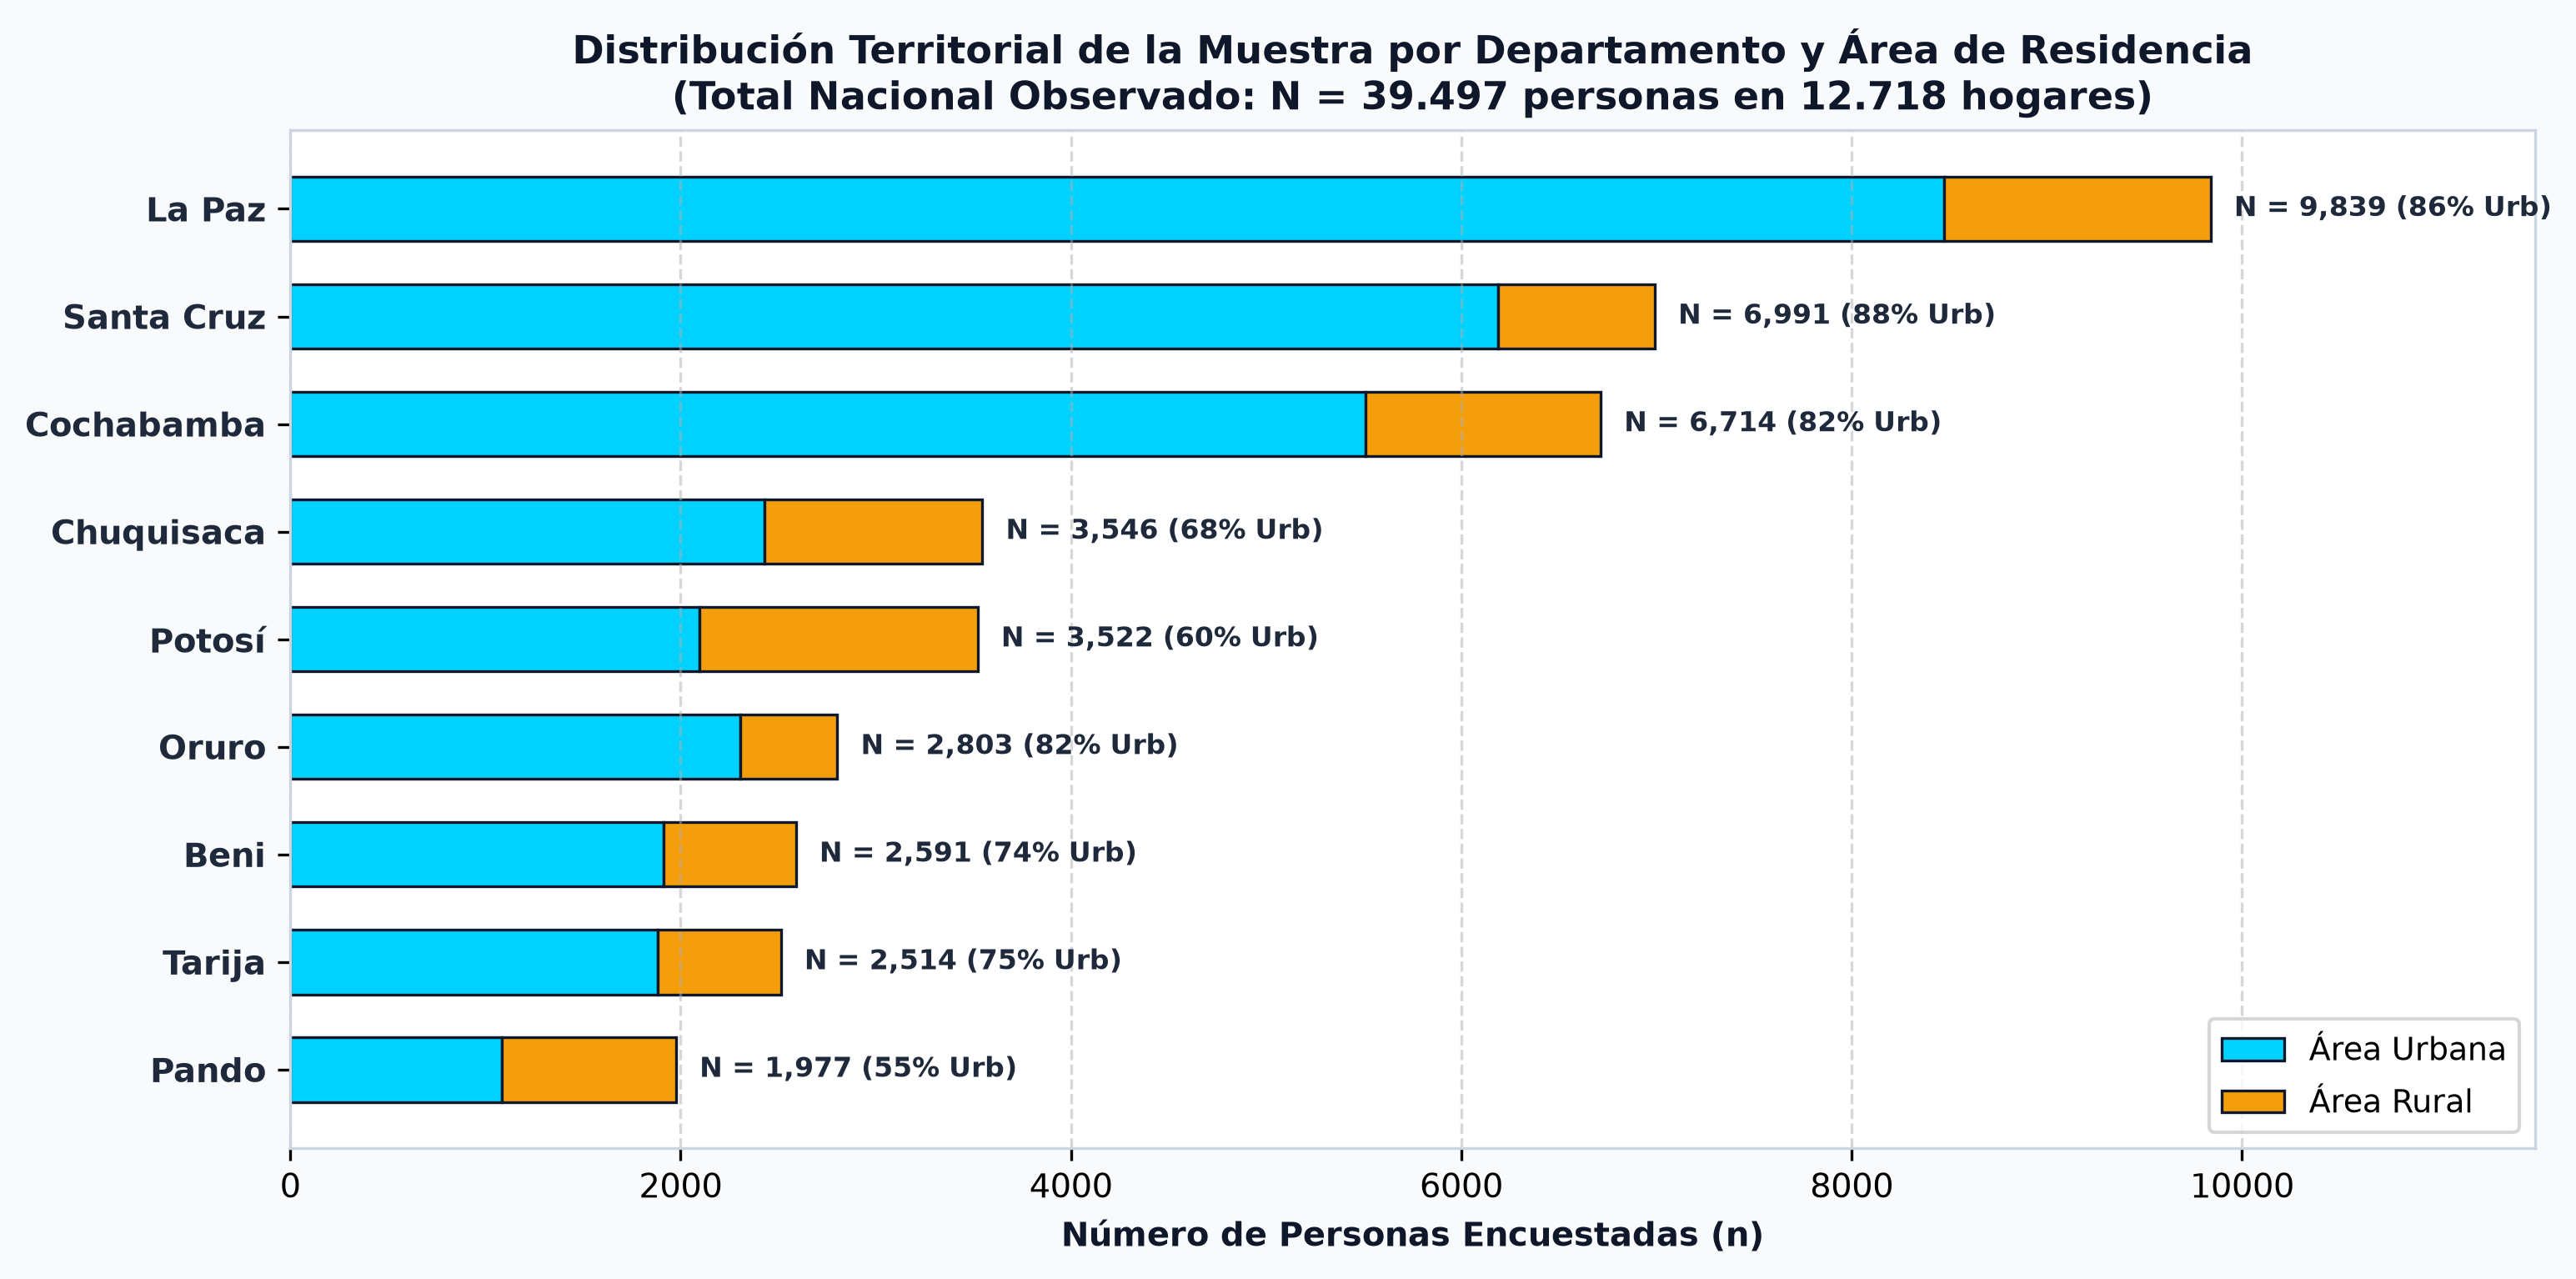
\includegraphics[width=0.98\textwidth]{figuras/fig4_distribucion_departamental.png}
\caption{Distribución territorial observada de la muestra por departamento y área de residencia}
\label{fig:distribucion_departamental}
\par\vspace{3pt}\parbox{0.98\textwidth}{\footnotesize\textit{Nota.} Conteo de registros válidos por departamento desagregados en área urbana y rural ($N = 39.497$ personas y $N_{\text{hog}} = 12.718$ hogares).}
\end{figure}

\subsection{Segmentación analítica: Las 11 vistas temáticas}
Para resolver el dilema entre conservar las 275 variables maestras y facilitar consultas estadísticas sobre subpoblaciones específicas, se derivaron 11 vistas temáticas no destructivas, alojadas en el subdirectorio \texttt{thematic\_views/} y sincronizadas mediante \texttt{views\_manifest.json}. La especificación formal de cada vista se presenta en la tabla \ref{tab:vistas_tematicas} y su cobertura comparativa en la figura \ref{fig:cobertura_vistas}.

\begin{table}[htbp]
\centering
\caption{Especificación técnica y criterios de elegibilidad de las 11 vistas temáticas}
\label{tab:vistas_tematicas}
\begin{tabularx}{\textwidth}{>{\raggedright\arraybackslash\small}p{2.85cm}>{\raggedright\arraybackslash\small}p{4.35cm}>{\raggedleft\arraybackslash\small}p{1.2cm}>{\raggedleft\arraybackslash\small}p{1.1cm}>{\raggedright\arraybackslash\small}X}
\toprule
\textbf{Identificador} & \textbf{Criterio / Filtro de elegibilidad oficial} & \textbf{Filas ($n$)} & \textbf{Cols} & \textbf{Universo de análisis} \\
\midrule
\texttt{\small demografia} & Muestra completa sin filtro restrictivo & 39.497 & 33 & Sociodemográfico general \\
\texttt{\small salud\_general} & Toda persona encuestada & 39.497 & 31 & Afiliación y centros \\
\texttt{\small salud\_fecund} & Mujeres de 13 a 50 años (\texttt{\small s01a\_02=2}) & 11.328 & 24 & Maternidad e historial \\
\texttt{\small salud\_infant} & Menores de 6 años de edad (\texttt{\small edad < 6}) & 3.434 & 10 & Desarrollo infantil \\
\texttt{\small salud\_bono} & Menores de 5 años de edad (\texttt{\small edad < 5}) & 2.781 & 12 & Vacunas y Bono Juana Azurduy \\
\texttt{\small educacion} & Población de 4 años o más (\texttt{\small edad $\ge$ 4}) & 37.354 & 43 & Asistencia y alfabetismo \\
\texttt{\small empleo\_pet} & Población en Edad de Trabajar (\texttt{\small edad $\ge$ 7}) & 35.366 & 121 & Actividad y ramas \\
\texttt{\small empleo\_sec} & Ocupados con 2do trabajo (\texttt{\small s04e\_25=1}) & 1.357 & 45 & Jornada secundaria \\
\texttt{\small ingresos\_nolab}& Todos los registros persona & 39.497 & 48 & Jubilaciones y bonos \\
\texttt{\small ingresos\_pob} & Todos los registros persona & 39.497 & 25 & Pobreza y per cápita \\
\texttt{\small hogar\_resumen} & Un registro por vivienda única (\texttt{\small folio}) & 12.718 & 18 & Agregados del hogar \\
\bottomrule
\end{tabularx}
\par\vspace{3pt}\parbox{\textwidth}{\footnotesize\textit{Nota.} La vista de hogar consolida variables invariantes por vivienda resolviendo ausencias sin colisión de valores observados. Fuente: \texttt{views\_manifest.json}.}
\end{table}

\begin{figure}[htbp]
\centering
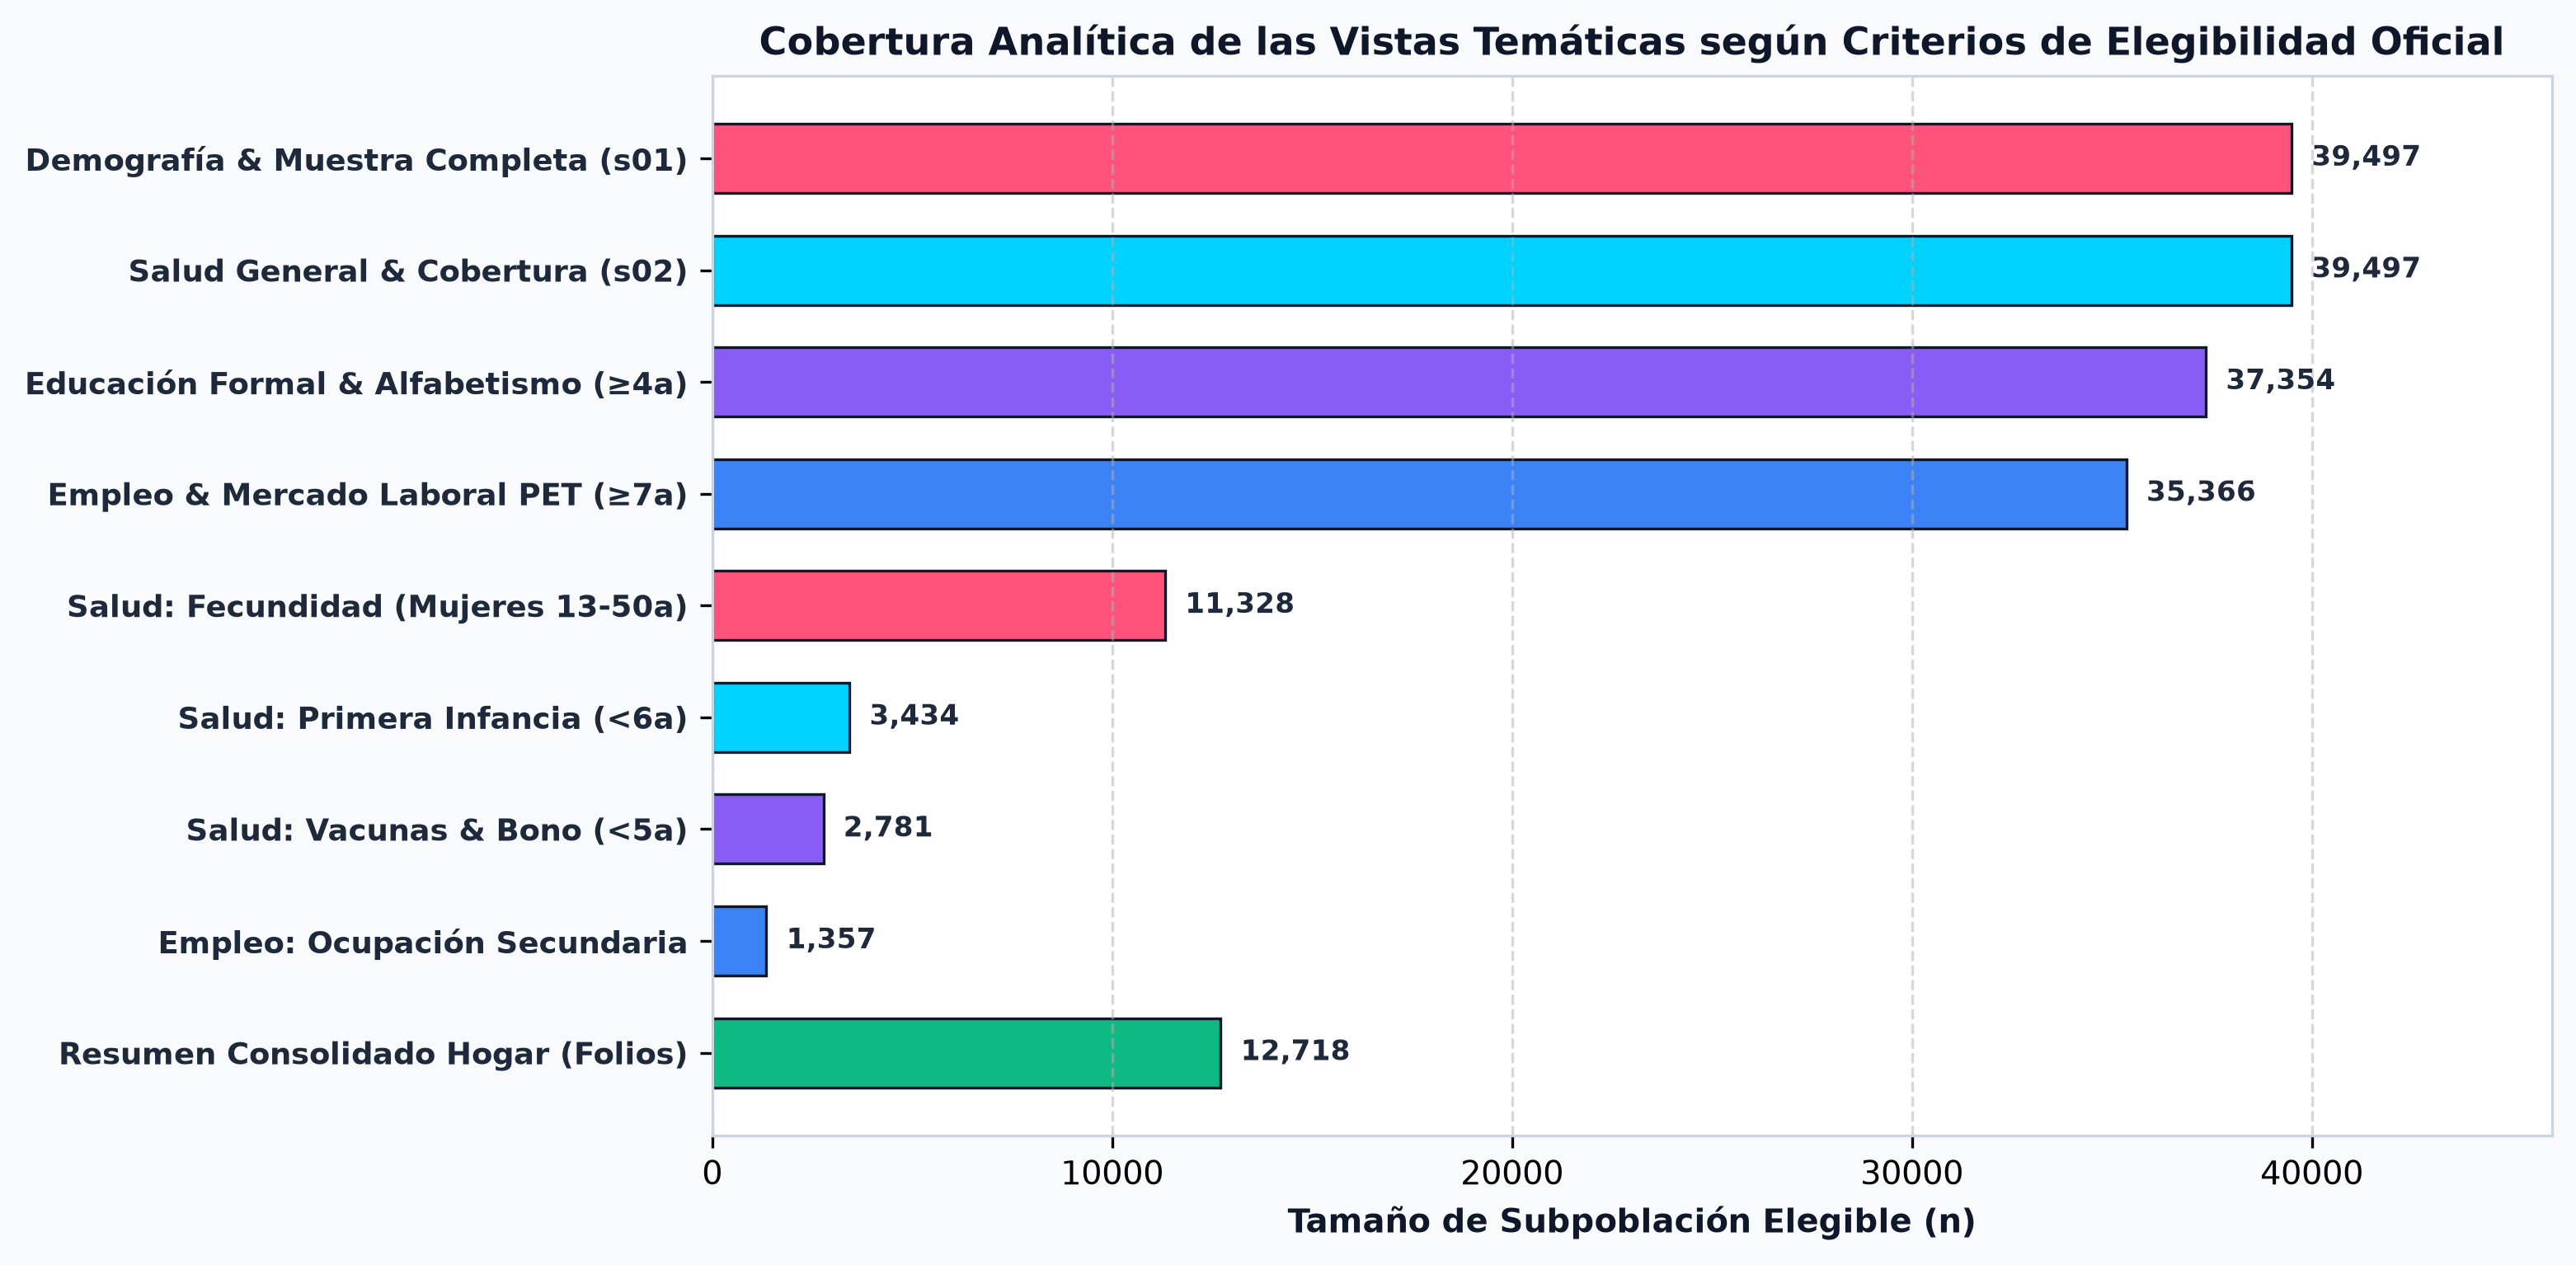
\includegraphics[width=0.98\textwidth]{figuras/fig6_cobertura_11_vistas.png}
\caption{Población elegible y cobertura analítica de las 11 vistas temáticas}
\label{fig:cobertura_vistas}
\par\vspace{3pt}\parbox{0.98\textwidth}{\footnotesize\textit{Nota.} Comparativa del tamaño muestral ($n$) retenido en cada módulo de acuerdo con los filtros de salto del cuestionario.}
\end{figure}

\subsection{Auditoría intrahogar en la muestra de control (QA)}
En la muestra determinista de control de 381 hogares (1.216 integrantes), se auditó la coherencia entre el número de personas observadas en el archivo y la variable declarada \texttt{totper}. Se constató que \texttt{totper} coincidió con las filas observadas en 69 hogares y registró diferencias en 312 casos. Al tratarse de una extensión local no documentada en el catálogo F27 del INE, se mantuvo intacta y no se utilizó como denominador en cálculos poblacionales, documentando la discrepancia en el registro de incidencias del catálogo.

\section{Dashboard interactivo y presentación analítica}

\subsection{Arquitectura del sistema web y desacoplamiento}
La interfaz analítica fue construida mediante el microframework Flask, complementada con plantillas modulares Jinja2 y estilos en CSS puro con arquitectura de variables y tokens de color personalizados (modo oscuro y claro). El sistema implementa un desacoplamiento estricto respecto al pipeline de datos: la aplicación no interactúa directamente con el archivo crudo ni ejecuta transformaciones sobre la marcha. En su lugar, el servicio central (\texttt{dataset\_service.py}) resuelve la versión publicada leyendo el archivo de registro JSON (\texttt{registry.json}), validando la huella SHA-256 del archivo Parquet o CSV antes de suministrar datos a las vistas.

\subsection{Módulos funcionales del sistema}
La suite interactiva se compone de tres módulos centrales (ilustrados en la figura \ref{fig:dashboard_suite}):

\begin{enumerate}[leftmargin=0.5in]
  \item \textbf{Resumen ejecutivo y control de calidad (\texttt{/dashboard/calidad}):} Expone métricas antes/después, tablas de frecuencia de ausencias por variable, trazabilidad de reglas de limpieza y confirmación de que la clave relacional \texttt{(folio, nro)} presenta cero colisiones.
  \item \textbf{Explorador de universos y diccionario (\texttt{/dashboard/universo}):} Permite navegar por las 11 vistas temáticas, consultando las etiquetas oficiales del INE F27, tasas de completitud por columna y criterios de exclusión de poblaciones no elegibles.
  \item \textbf{Distribución regional y mapa interactivo (\texttt{/dashboard/region}):} Cartografía digital oficial del Estado Plurinacional de Bolivia basada en polígonos vectoriales SVG de alta precisión para los nueve departamentos.
\end{enumerate}

\begin{figure}[htbp]
\centering
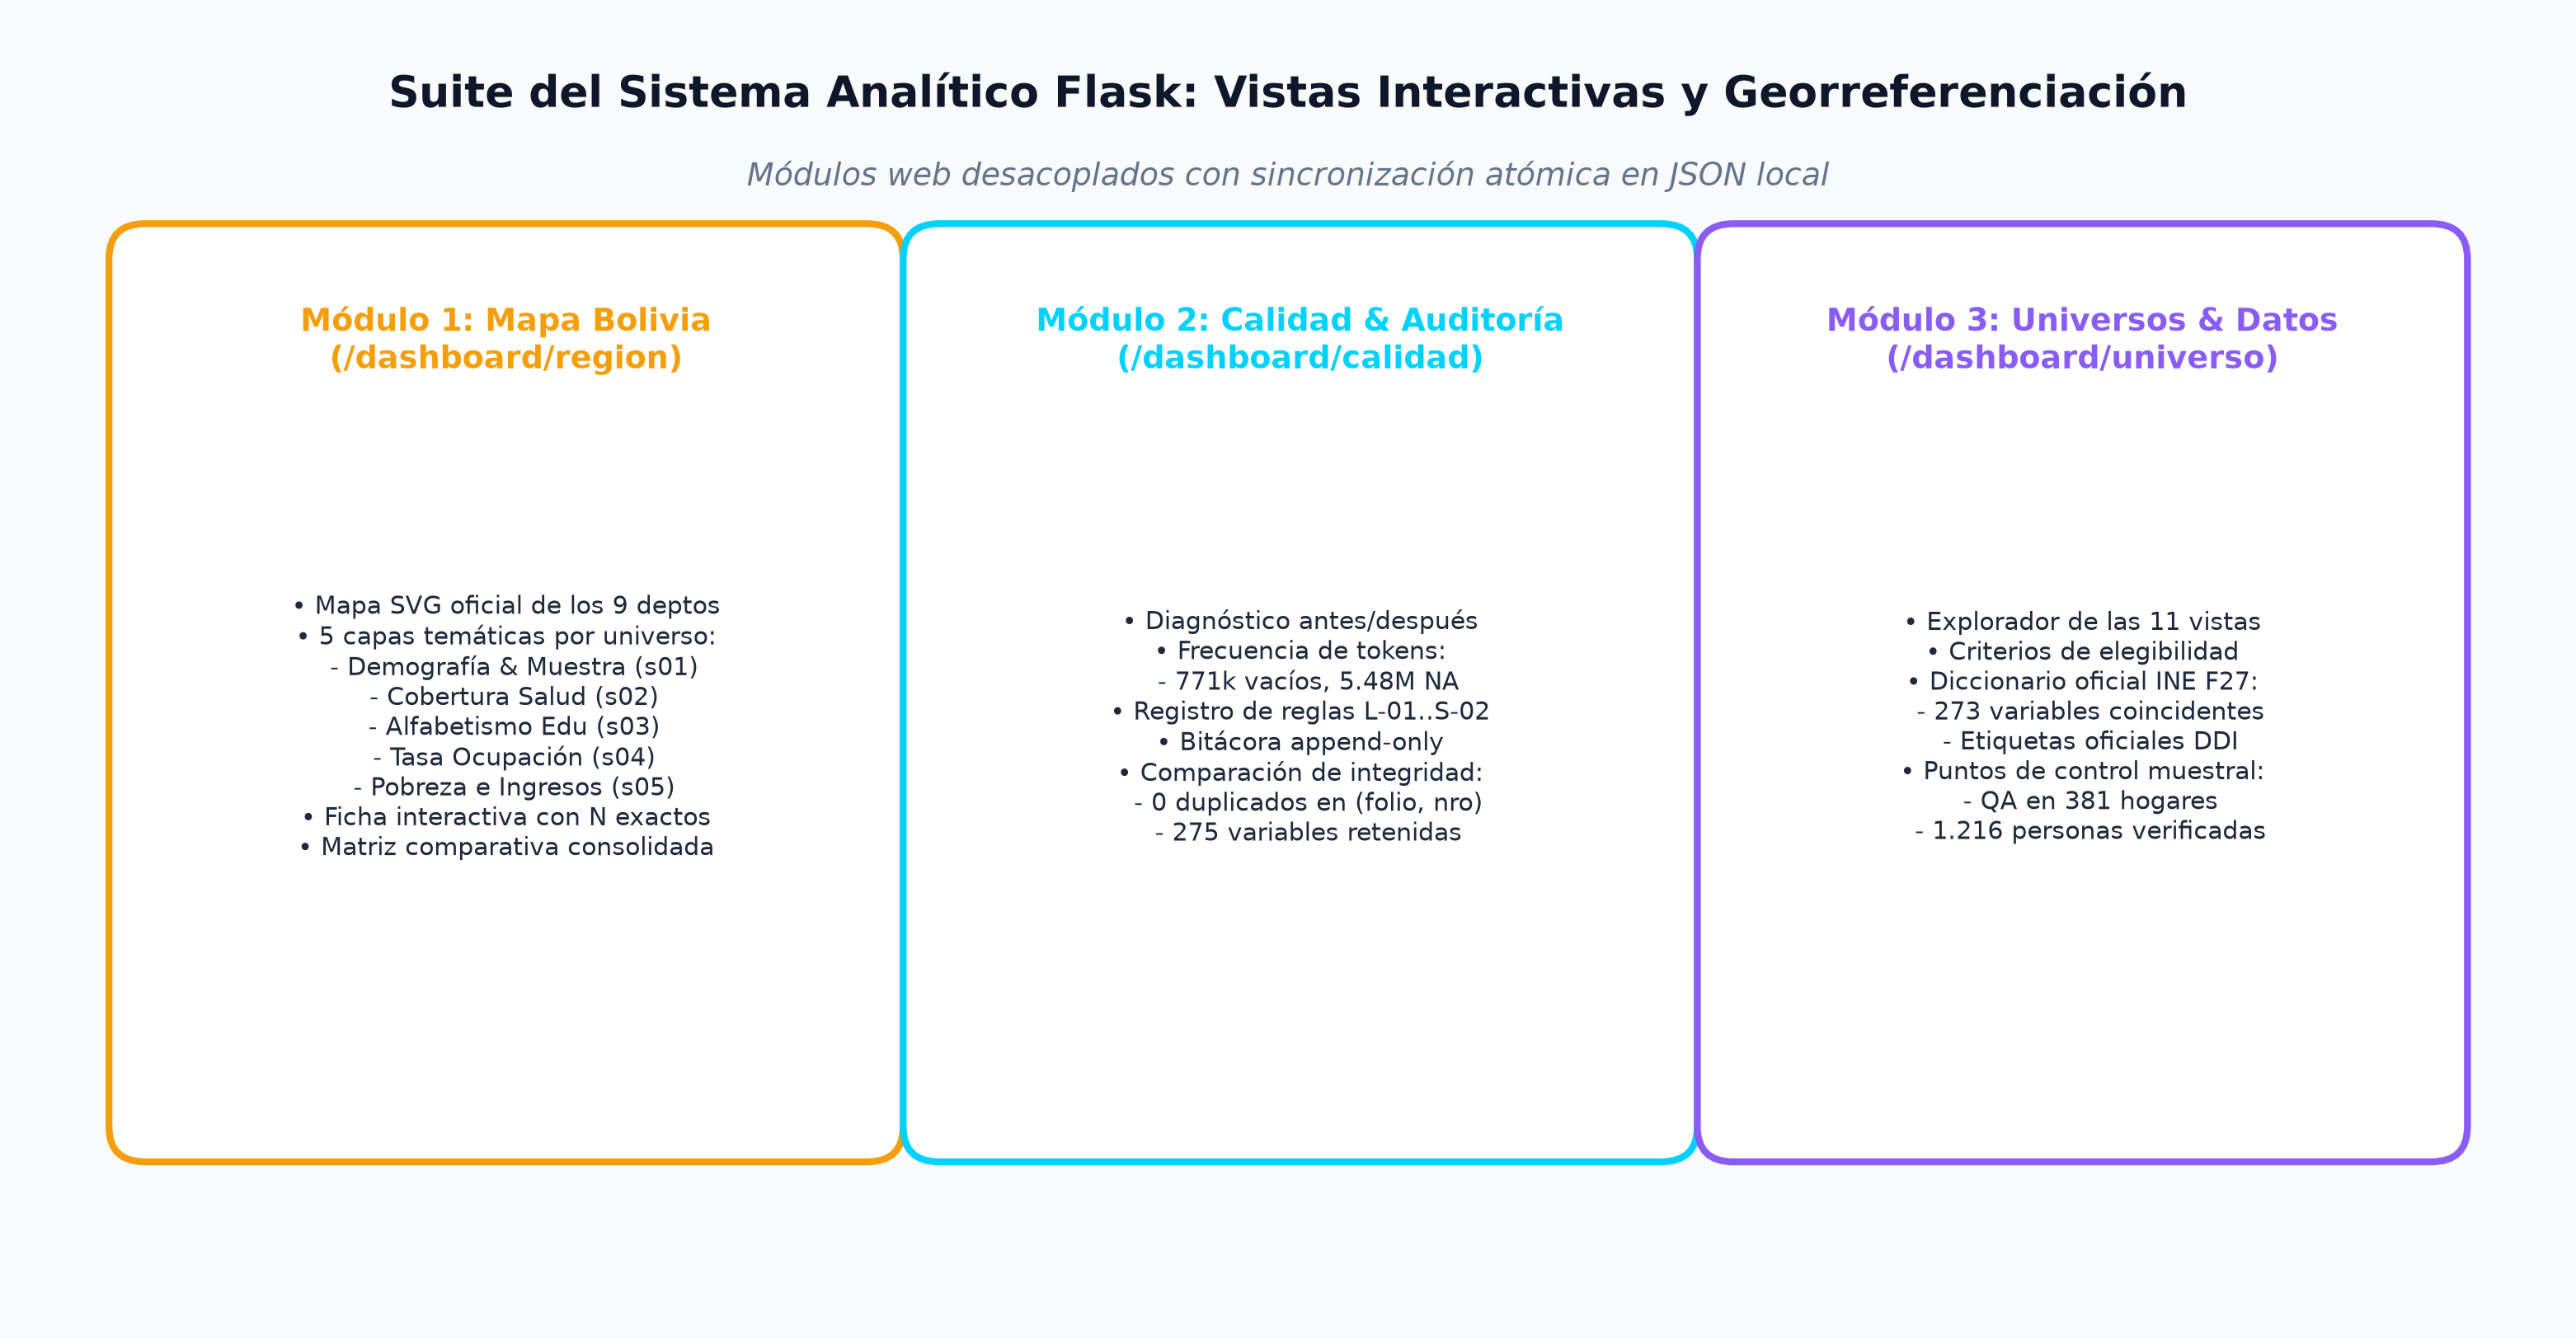
\includegraphics[width=0.98\textwidth]{figuras/fig7_dashboard_suite_capturas.png}
\caption{Suite interactiva del sistema analítico Flask: Módulos de Georreferenciación, Calidad y Universos}
\label{fig:dashboard_suite}
\par\vspace{3pt}\parbox{0.98\textwidth}{\footnotesize\textit{Nota.} Estructura modular del front-end analítico: módulo regional con mapa SVG de Bolivia, módulo de auditoría de calidad y explorador de las 11 vistas temáticas.}
\end{figure}

\subsection{Cartografía interactiva y consolidación departamental}
A diferencia de implementaciones preliminares que empleaban métricas demostrativas, el módulo regional fue completamente actualizado para consumir las cantidades estadísticas exactas calculadas directamente desde el maestro \texttt{persona\_clean\_master.parquet}. 

El mapa interactivo permite activar cinco capas temáticas dinámicas:
\begin{itemize}[leftmargin=0.5in]
  \item \textit{División Departamental Oficial (Capa Política):} Mapeo cromático de los 9 departamentos.
  \item \textit{Demografía \& Muestra ($s01$):} Densidad observada de personas y hogares encuestados.
  \item \textit{Universo Salud ($s02$):} Tasa de cobertura de seguro médico (SUS, Cajas de Salud y privados).
  \item \textit{Universo Educación ($s03$):} Tasa de alfabetismo en personas de 15 años o más.
  \item \textit{Universo Empleo ($s04$):} Tasa de ocupación en la Población en Edad de Trabajar (PET $\ge 7$ años).
  \item \textit{Universo Ingresos ($s05$):} Incidencia de pobreza moderada observada.
\end{itemize}

Al interactuar con cualquier departamento en el mapa SVG o en la tabla, el panel lateral actualiza dinámicamente las cifras de muestra observada, desglose urbano/rural, población femenina en edad fértil (MEF 13--50 años), niñez asistida y mediana del ingreso laboral líquido. La síntesis de estas métricas se presenta en la tabla \ref{tab:matriz_departamental}.

\begin{table}[htbp]
\centering
\caption{Matriz consolidada de la muestra por departamento y universos de la encuesta}
\label{tab:matriz_departamental}
\begin{tabularx}{\textwidth}{>{\raggedright\arraybackslash\small}p{2.1cm}>{\raggedleft\arraybackslash\small}p{1.35cm}>{\raggedleft\arraybackslash\small}p{1.35cm}>{\raggedleft\arraybackslash\small}p{1.75cm}>{\raggedleft\arraybackslash\small}p{1.85cm}>{\raggedleft\arraybackslash\small}p{1.65cm}>{\raggedleft\arraybackslash\small}X}
\toprule
\textbf{Depto} & \textbf{Muestra ($N$)} & \textbf{Hogares} & \textbf{Con Seguro ($s02$)} & \textbf{Alfabetos $\ge$15a ($s03$)} & \textbf{Ocupados PET ($s04$)} & \textbf{Pobres ($s05$)} \\
\midrule
Chuquisaca & 3.546 & 1.130 & 2.681 (75,6\%) & 2.351 (89,6\%) & 2.075 (64,6\%) & 1.738 (49,0\%) \\
La Paz & 9.839 & 3.251 & 6.484 (65,9\%) & 7.350 (97,9\%) & 5.411 (60,5\%) & 4.300 (43,7\%) \\
Cochabamba & 6.714 & 2.166 & 4.915 (73,2\%) & 4.972 (96,6\%) & 3.612 (59,3\%) & 2.253 (33,6\%) \\
Oruro & 2.803 & 952 & 2.189 (78,1\%) & 2.048 (97,1\%) & 1.610 (63,8\%) & 995 (35,5\%) \\
Potosí & 3.522 & 1.133 & 2.877 (81,7\%) & 2.311 (91,1\%) & 1.894 (61,0\%) & 1.972 (56,0\%) \\
Tarija & 2.514 & 832 & 2.277 (90,6\%) & 1.817 (95,7\%) & 1.378 (60,6\%) & 802 (31,9\%) \\
Santa Cruz & 6.991 & 2.028 & 4.153 (59,4\%) & 5.021 (98,0\%) & 3.788 (60,8\%) & 1.587 (22,7\%) \\
Beni & 2.591 & 718 & 2.044 (78,9\%) & 1.789 (97,8\%) & 1.332 (58,3\%) & 933 (36,0\%) \\
Pando & 1.977 & 508 & 1.479 (74,8\%) & 1.305 (98,3\%) & 1.209 (71,0\%) & 731 (37,0\%) \\
\midrule
\textbf{Total} & \textbf{39.497} & \textbf{12.718} & \textbf{29.099 (73,7\%)} & \textbf{28.964 (96,3\%)} & \textbf{22.309 (61,3\%)} & \textbf{15.311 (38,8\%)} \\
\bottomrule
\end{tabularx}
\par\vspace{3pt}\parbox{\textwidth}{\footnotesize\textit{Nota.} Conteos exactos de la muestra observada. Las tasas departamentales corresponden a la población elegible evaluada en cada módulo de la encuesta. Fuente: \texttt{departamentos\_full\_stats.json}.}
\end{table}

\subsection{Políticas de privacidad y supresión de celdas pequeñas}
Para evitar la reidentificación de personas o informantes en celdas estadísticas desagregadas, el servicio de visualización aplica una regla estricta de supresión de umbral: cualquier categoría con menos de 10 registros individuales observados se suprime de los gráficos públicos. Adicionalmente, se ejecuta supresión complementaria en la categoría de menor frecuencia contigua para impedir que el usuario deduzca el valor oculto a partir del total marginal $N$.

\section{Discusión}

\subsection{Integridad estructural frente al mito de la limpieza destructiva}
Los resultados obtenidos demuestran un avance metodológico sustancial respecto a los enfoques convencionales de preparación de datos: el dataset maestro conserva íntegramente sus 275 variables y 39.497 filas, sin recurrir a la supresión arbitraria de columnas dispersas ni a la imputación algorítmica ciega de valores faltantes. 

La decisión de reclasificar la regla L-80 como una alerta meramente informativa en lugar de un mecanismo de eliminación automática fue plenamente respaldada por la evidencia empírica. El análisis demostró que en encuestas de hogares, la ausencia global agrega poblaciones heterogéneas; excluir atributos con más del 80\% de valores \texttt{NA} habría destruido variables críticas de la economía laboral, tales como el salario líquido (\texttt{s04c\_17a}) o las características del empleo secundario (\texttt{s04e\_26\_cod}), las cuales exhiben tasas de respuesta superiores al 99\% cuando se calculan sobre su universo elegible documentado.

\subsection{El concepto de dataset limpio y las limitaciones semánticas}
En consonancia con los principios de calidad de datos, es imperativo distinguir entre \textit{integridad estructural} y \textit{depuración semántica integral}. El artefacto \texttt{persona\_clean\_master.parquet} es un dataset estructuralmente impecable: no contiene colisiones de clave, registros truncados ni tipos incompatibles, y sus alteraciones físicas se limitan a tres celdas biológicamente imposibles en horas semanales (regla S-01) y a la normalización de cadenas de texto libre (regla S-02). 

No obstante, no puede afirmarse que la matriz esté 100\% depurada en términos de negocio o semántica oficial. Como se identificó en la conciliación con el catálogo F27 del INE, existen diferencias de 12 registros (39.497 en la copia de trabajo frente a 39.485 en el estándar público), tres atributos oficiales no presentes localmente y dos extensiones locales sin diccionario confirmado (\texttt{s05c\_09e} y \texttt{totper}). Por ello, clasificar la versión publicada como \texttt{published\_internal\_with\_semantic\_limitations} constituye un acto de honestidad científica indispensable.

\subsection{Diseño muestral, representatividad y límites inferenciales}
La muestra de 39.497 personas en 12.718 hogares observados en los nueve departamentos del país no representa una muestra aleatoria simple (M.A.S.), sino un diseño estratificado y por conglomerados (UPM). Como consecuencia directa:
\begin{itemize}[leftmargin=0.5in]
  \item Existe una clara sobre-representación intencional de departamentos pequeños (como Pando con 1.977 encuestados para una población proyectada de 175 mil hab., frente a Santa Cruz con 6.991 encuestados para más de 3,5 millones de hab.).
  \item Las tasas observadas presentadas en el dashboard deben interpretarse estrictamente como indicadores de la muestra encuestada. La extrapolación hacia el total nacional de 12,4 millones de habitantes requiere expandir mediante la variable de ponderación \texttt{factor} y aplicar métodos de estimación de varianza compatibles con el diseño de la encuesta (como linealización por series de Taylor o réplicas bootstrap).
\end{itemize}

\subsection{Consolidación de la vista regional}
La actualización del módulo geográfico en la aplicación web resolvió la desconexión documentada en revisiones previas. Al vincular el mapa vectorial SVG de Bolivia directamente con las métricas observadas consolidadas en \texttt{departamentos\_full\_stats.json}, el usuario dispone de un contraste regional transparente y fidedigno, distinguiendo con claridad entre el conteo muestral observado ($n$) y el universo de referencia elegible para cada dimensión de salud, educación, empleo y pobreza.

\section{Conclusiones y trabajo futuro}

\subsection{Conclusiones del proyecto}
El desarrollo del proyecto permitió establecer un estándar de ingeniería y minería de datos riguroso, reproducible y éticamente responsable sobre el microdato sociodemográfico \texttt{data/persona.csv}. Se destacan los siguientes logros fundamentales:

\begin{enumerate}[leftmargin=0.5in]
  \item \textbf{Preservación estricta de la fuente y reproducibilidad criptográfica:} Se mantuvo la inmutabilidad absoluta de \texttt{data/persona.csv}, respaldada por su hash SHA-256. Toda ejecución del pipeline generó artefactos versionados e independientes, materializando una versión maestra limpia (\texttt{persona\_clean\_master.parquet}) con las 39.497 filas y 275 columnas intactas.
  \item \textbf{Superación del paradigma de limpieza destructiva:} Se demostró teórica y empíricamente que la eliminación ciega de variables con alta tasa de ausencia técnica (regla L-80) o la imputación mecánica de medias sobre atributos condicionales destruyen la semántica de las encuestas por muestreo. La conservación íntegra del esquema permitió retener información crucial sobre empleo asalariado e ingresos secundarios.
  \item \textbf{Aplicación de reglas semánticas auditables:} Se ejecutaron únicamente transformaciones con fundamento verificable: validación de unicidad de la tupla relacional \texttt{(folio, nro)}, tipado estricto, corrección de frontera física en la regla S-01 (reasignación a \texttt{NA} de 3 celdas con jornadas mayores a 168 horas semanales) y estandarización lingüística en la regla S-02 (12.516 celdas en minúsculas en 13 variables de especificación abierta), con registro detallado en bitácora append-only.
  \item \textbf{Estructuración de 11 vistas temáticas especializadas:} La segmentación no destructiva de la matriz según poblaciones elegibles (educación $\ge 4$ años, empleo $\ge 7$ años, fecundidad, niñez, ingresos y agregados de hogar) resolvió el compromiso entre integridad global y eficiencia en consultas estadísticas focalizadas.
  \item \textbf{Arquitectura desacoplada y despliegue interactivo:} Se construyó una aplicación web funcional en Flask con persistencia atómica en documentos JSON locales (sin sobrecostos de configuración en bases de datos relacionales), integrando un mapa interactivo de Bolivia con división oficial de los 9 departamentos que consume datos observados fidedignos, con arquitectura portable lista para despliegue continuo en entornos productivos.
\end{enumerate}

\subsection{Trabajo futuro y recomendaciones}
Para las fases subsiguientes del ciclo de minería de datos, se recomienda:
\begin{itemize}[leftmargin=0.5in]
  \item \textbf{Conciliación formal de la procedencia:} Gestionar con la entidad emisora (INE) la versión oficial del formulario y manual de codificación para resolver la naturaleza de los 12 casos divergentes y las extensiones locales (\texttt{totper} y \texttt{s05c\_09e}).
  \item \textbf{Modelado inferencial con diseño de encuesta:} Incorporar rutinas estadísticas en Python (mediante librerías especializadas como \texttt{statsmodels} o \texttt{samplics}) que utilicen los estratos, UPM y el factor de expansión (\texttt{factor}) para calcular errores estándar, intervalos de confianza y contrastes de hipótesis representativos de la población boliviana.
  \item \textbf{Modelado predictivo y de agrupamiento (KDD Fase 4):} Con una base de datos limpia y segmentada, abordar tareas de segmentación socioeconómica mediante clustering no supervisado (K-Means, GMM) y modelos de clasificación para la predicción de vulnerabilidad o inserción laboral informal.
\end{itemize}


\newpage
\printbibliography[title={Referencias}]

\appendix
\section{Reproducibilidad y artefactos consultados}
La verificación documentada para esta entrega se ejecuta desde la raíz del repositorio. El comando de pruebas registrado fue:
\begin{quote}\small\texttt{python -m unittest discover -s tests -v}\end{quote}
En el entorno usado el ejecutable global de Python 3.12 fue invocado mediante su ruta absoluta. El resultado más reciente registrado para el cambio de etiquetas del dashboard fue de 16 pruebas aprobadas. Las pruebas son sintéticas y verifican comportamientos del código; no son análisis estadísticos adicionales de los microdatos.

Version interna examinada: persona-317279aafe9023a2 (39.497 filas por 275 columnas). Sus artefactos versionados y la documentacion fuente se conservan en el repositorio. Consultar las secciones de metodologia, conciliacion, auditoria semantica, validacion, analisis exploratorio y dashboard.

\end{document}
